% TMLR submission draft v2 -- Transactions on Machine Learning Research
% Style: tmlr.sty / tmlr.bst (github.com/JmlrOrg/tmlr-style-file, downloaded 2026-10-15).
% Submission mode: \usepackage{tmlr} hides the author block (double-blind). Do NOT use [preprint]/[accepted]
% for the OpenReview submission. No page limit; length must be justified by content.
%
% Build:  tectonic -X compile main.tex   (or pdflatex -> bibtex -> pdflatex x2)
%
% v2 (2026-11-01): claim-centric structure; results of the follow-up experiments of 2026-11-01
% (training-free grid V{v}-A{k}, 20k current/ego-only heads, pass-1 noise seeds, quiet-host latency).
% v1.1 is kept in archive/main_v1.1.tex.
%
% Anonymity checklist before submission: no author names, no institution, no GitHub URL with a user name,
% no server names, no links to the Korean technical report. Supplementary code (<=100 MB zip) must be anonymized.

\documentclass[10pt]{article}
\usepackage{tmlr}
% \usepackage[accepted]{tmlr}   % camera-ready
% \usepackage[preprint]{tmlr}   % arXiv version (de-anonymized)

%%%%% NEW MATH DEFINITIONS %%%%%

\usepackage{amsmath,amsfonts,bm}

% Mark sections of captions for referring to divisions of figures
\newcommand{\figleft}{{\em (Left)}}
\newcommand{\figcenter}{{\em (Center)}}
\newcommand{\figright}{{\em (Right)}}
\newcommand{\figtop}{{\em (Top)}}
\newcommand{\figbottom}{{\em (Bottom)}}
\newcommand{\captiona}{{\em (a)}}
\newcommand{\captionb}{{\em (b)}}
\newcommand{\captionc}{{\em (c)}}
\newcommand{\captiond}{{\em (d)}}

% Highlight a newly defined term
\newcommand{\newterm}[1]{{\bf #1}}


% Figure reference, lower-case.
\def\figref#1{figure~\ref{#1}}
% Figure reference, capital. For start of sentence
\def\Figref#1{Figure~\ref{#1}}
\def\twofigref#1#2{figures \ref{#1} and \ref{#2}}
\def\quadfigref#1#2#3#4{figures \ref{#1}, \ref{#2}, \ref{#3} and \ref{#4}}
% Section reference, lower-case.
\def\secref#1{section~\ref{#1}}
% Section reference, capital.
\def\Secref#1{Section~\ref{#1}}
% Reference to two sections.
\def\twosecrefs#1#2{sections \ref{#1} and \ref{#2}}
% Reference to three sections.
\def\secrefs#1#2#3{sections \ref{#1}, \ref{#2} and \ref{#3}}
% Reference to an equation, lower-case.
\def\eqref#1{equation~\ref{#1}}
% Reference to an equation, upper case
\def\Eqref#1{Equation~\ref{#1}}
% A raw reference to an equation---avoid using if possible
\def\plaineqref#1{\ref{#1}}
% Reference to a chapter, lower-case.
\def\chapref#1{chapter~\ref{#1}}
% Reference to an equation, upper case.
\def\Chapref#1{Chapter~\ref{#1}}
% Reference to a range of chapters
\def\rangechapref#1#2{chapters\ref{#1}--\ref{#2}}
% Reference to an algorithm, lower-case.
\def\algref#1{algorithm~\ref{#1}}
% Reference to an algorithm, upper case.
\def\Algref#1{Algorithm~\ref{#1}}
\def\twoalgref#1#2{algorithms \ref{#1} and \ref{#2}}
\def\Twoalgref#1#2{Algorithms \ref{#1} and \ref{#2}}
% Reference to a part, lower case
\def\partref#1{part~\ref{#1}}
% Reference to a part, upper case
\def\Partref#1{Part~\ref{#1}}
\def\twopartref#1#2{parts \ref{#1} and \ref{#2}}

\def\ceil#1{\lceil #1 \rceil}
\def\floor#1{\lfloor #1 \rfloor}
\def\1{\bm{1}}
\newcommand{\train}{\mathcal{D}}
\newcommand{\valid}{\mathcal{D_{\mathrm{valid}}}}
\newcommand{\test}{\mathcal{D_{\mathrm{test}}}}

\def\eps{{\epsilon}}


% Random variables
\def\reta{{\textnormal{$\eta$}}}
\def\ra{{\textnormal{a}}}
\def\rb{{\textnormal{b}}}
\def\rc{{\textnormal{c}}}
\def\rd{{\textnormal{d}}}
\def\re{{\textnormal{e}}}
\def\rf{{\textnormal{f}}}
\def\rg{{\textnormal{g}}}
\def\rh{{\textnormal{h}}}
\def\ri{{\textnormal{i}}}
\def\rj{{\textnormal{j}}}
\def\rk{{\textnormal{k}}}
\def\rl{{\textnormal{l}}}
% rm is already a command, just don't name any random variables m
\def\rn{{\textnormal{n}}}
\def\ro{{\textnormal{o}}}
\def\rp{{\textnormal{p}}}
\def\rq{{\textnormal{q}}}
\def\rr{{\textnormal{r}}}
\def\rs{{\textnormal{s}}}
\def\rt{{\textnormal{t}}}
\def\ru{{\textnormal{u}}}
\def\rv{{\textnormal{v}}}
\def\rw{{\textnormal{w}}}
\def\rx{{\textnormal{x}}}
\def\ry{{\textnormal{y}}}
\def\rz{{\textnormal{z}}}

% Random vectors
\def\rvepsilon{{\mathbf{\epsilon}}}
\def\rvtheta{{\mathbf{\theta}}}
\def\rva{{\mathbf{a}}}
\def\rvb{{\mathbf{b}}}
\def\rvc{{\mathbf{c}}}
\def\rvd{{\mathbf{d}}}
\def\rve{{\mathbf{e}}}
\def\rvf{{\mathbf{f}}}
\def\rvg{{\mathbf{g}}}
\def\rvh{{\mathbf{h}}}
\def\rvu{{\mathbf{i}}}
\def\rvj{{\mathbf{j}}}
\def\rvk{{\mathbf{k}}}
\def\rvl{{\mathbf{l}}}
\def\rvm{{\mathbf{m}}}
\def\rvn{{\mathbf{n}}}
\def\rvo{{\mathbf{o}}}
\def\rvp{{\mathbf{p}}}
\def\rvq{{\mathbf{q}}}
\def\rvr{{\mathbf{r}}}
\def\rvs{{\mathbf{s}}}
\def\rvt{{\mathbf{t}}}
\def\rvu{{\mathbf{u}}}
\def\rvv{{\mathbf{v}}}
\def\rvw{{\mathbf{w}}}
\def\rvx{{\mathbf{x}}}
\def\rvy{{\mathbf{y}}}
\def\rvz{{\mathbf{z}}}

% Elements of random vectors
\def\erva{{\textnormal{a}}}
\def\ervb{{\textnormal{b}}}
\def\ervc{{\textnormal{c}}}
\def\ervd{{\textnormal{d}}}
\def\erve{{\textnormal{e}}}
\def\ervf{{\textnormal{f}}}
\def\ervg{{\textnormal{g}}}
\def\ervh{{\textnormal{h}}}
\def\ervi{{\textnormal{i}}}
\def\ervj{{\textnormal{j}}}
\def\ervk{{\textnormal{k}}}
\def\ervl{{\textnormal{l}}}
\def\ervm{{\textnormal{m}}}
\def\ervn{{\textnormal{n}}}
\def\ervo{{\textnormal{o}}}
\def\ervp{{\textnormal{p}}}
\def\ervq{{\textnormal{q}}}
\def\ervr{{\textnormal{r}}}
\def\ervs{{\textnormal{s}}}
\def\ervt{{\textnormal{t}}}
\def\ervu{{\textnormal{u}}}
\def\ervv{{\textnormal{v}}}
\def\ervw{{\textnormal{w}}}
\def\ervx{{\textnormal{x}}}
\def\ervy{{\textnormal{y}}}
\def\ervz{{\textnormal{z}}}

% Random matrices
\def\rmA{{\mathbf{A}}}
\def\rmB{{\mathbf{B}}}
\def\rmC{{\mathbf{C}}}
\def\rmD{{\mathbf{D}}}
\def\rmE{{\mathbf{E}}}
\def\rmF{{\mathbf{F}}}
\def\rmG{{\mathbf{G}}}
\def\rmH{{\mathbf{H}}}
\def\rmI{{\mathbf{I}}}
\def\rmJ{{\mathbf{J}}}
\def\rmK{{\mathbf{K}}}
\def\rmL{{\mathbf{L}}}
\def\rmM{{\mathbf{M}}}
\def\rmN{{\mathbf{N}}}
\def\rmO{{\mathbf{O}}}
\def\rmP{{\mathbf{P}}}
\def\rmQ{{\mathbf{Q}}}
\def\rmR{{\mathbf{R}}}
\def\rmS{{\mathbf{S}}}
\def\rmT{{\mathbf{T}}}
\def\rmU{{\mathbf{U}}}
\def\rmV{{\mathbf{V}}}
\def\rmW{{\mathbf{W}}}
\def\rmX{{\mathbf{X}}}
\def\rmY{{\mathbf{Y}}}
\def\rmZ{{\mathbf{Z}}}

% Elements of random matrices
\def\ermA{{\textnormal{A}}}
\def\ermB{{\textnormal{B}}}
\def\ermC{{\textnormal{C}}}
\def\ermD{{\textnormal{D}}}
\def\ermE{{\textnormal{E}}}
\def\ermF{{\textnormal{F}}}
\def\ermG{{\textnormal{G}}}
\def\ermH{{\textnormal{H}}}
\def\ermI{{\textnormal{I}}}
\def\ermJ{{\textnormal{J}}}
\def\ermK{{\textnormal{K}}}
\def\ermL{{\textnormal{L}}}
\def\ermM{{\textnormal{M}}}
\def\ermN{{\textnormal{N}}}
\def\ermO{{\textnormal{O}}}
\def\ermP{{\textnormal{P}}}
\def\ermQ{{\textnormal{Q}}}
\def\ermR{{\textnormal{R}}}
\def\ermS{{\textnormal{S}}}
\def\ermT{{\textnormal{T}}}
\def\ermU{{\textnormal{U}}}
\def\ermV{{\textnormal{V}}}
\def\ermW{{\textnormal{W}}}
\def\ermX{{\textnormal{X}}}
\def\ermY{{\textnormal{Y}}}
\def\ermZ{{\textnormal{Z}}}

% Vectors
\def\vzero{{\bm{0}}}
\def\vone{{\bm{1}}}
\def\vmu{{\bm{\mu}}}
\def\vtheta{{\bm{\theta}}}
\def\va{{\bm{a}}}
\def\vb{{\bm{b}}}
\def\vc{{\bm{c}}}
\def\vd{{\bm{d}}}
\def\ve{{\bm{e}}}
\def\vf{{\bm{f}}}
\def\vg{{\bm{g}}}
\def\vh{{\bm{h}}}
\def\vi{{\bm{i}}}
\def\vj{{\bm{j}}}
\def\vk{{\bm{k}}}
\def\vl{{\bm{l}}}
\def\vm{{\bm{m}}}
\def\vn{{\bm{n}}}
\def\vo{{\bm{o}}}
\def\vp{{\bm{p}}}
\def\vq{{\bm{q}}}
\def\vr{{\bm{r}}}
\def\vs{{\bm{s}}}
\def\vt{{\bm{t}}}
\def\vu{{\bm{u}}}
\def\vv{{\bm{v}}}
\def\vw{{\bm{w}}}
\def\vx{{\bm{x}}}
\def\vy{{\bm{y}}}
\def\vz{{\bm{z}}}

% Elements of vectors
\def\evalpha{{\alpha}}
\def\evbeta{{\beta}}
\def\evepsilon{{\epsilon}}
\def\evlambda{{\lambda}}
\def\evomega{{\omega}}
\def\evmu{{\mu}}
\def\evpsi{{\psi}}
\def\evsigma{{\sigma}}
\def\evtheta{{\theta}}
\def\eva{{a}}
\def\evb{{b}}
\def\evc{{c}}
\def\evd{{d}}
\def\eve{{e}}
\def\evf{{f}}
\def\evg{{g}}
\def\evh{{h}}
\def\evi{{i}}
\def\evj{{j}}
\def\evk{{k}}
\def\evl{{l}}
\def\evm{{m}}
\def\evn{{n}}
\def\evo{{o}}
\def\evp{{p}}
\def\evq{{q}}
\def\evr{{r}}
\def\evs{{s}}
\def\evt{{t}}
\def\evu{{u}}
\def\evv{{v}}
\def\evw{{w}}
\def\evx{{x}}
\def\evy{{y}}
\def\evz{{z}}

% Matrix
\def\mA{{\bm{A}}}
\def\mB{{\bm{B}}}
\def\mC{{\bm{C}}}
\def\mD{{\bm{D}}}
\def\mE{{\bm{E}}}
\def\mF{{\bm{F}}}
\def\mG{{\bm{G}}}
\def\mH{{\bm{H}}}
\def\mI{{\bm{I}}}
\def\mJ{{\bm{J}}}
\def\mK{{\bm{K}}}
\def\mL{{\bm{L}}}
\def\mM{{\bm{M}}}
\def\mN{{\bm{N}}}
\def\mO{{\bm{O}}}
\def\mP{{\bm{P}}}
\def\mQ{{\bm{Q}}}
\def\mR{{\bm{R}}}
\def\mS{{\bm{S}}}
\def\mT{{\bm{T}}}
\def\mU{{\bm{U}}}
\def\mV{{\bm{V}}}
\def\mW{{\bm{W}}}
\def\mX{{\bm{X}}}
\def\mY{{\bm{Y}}}
\def\mZ{{\bm{Z}}}
\def\mBeta{{\bm{\beta}}}
\def\mPhi{{\bm{\Phi}}}
\def\mLambda{{\bm{\Lambda}}}
\def\mSigma{{\bm{\Sigma}}}

% Tensor
\DeclareMathAlphabet{\mathsfit}{\encodingdefault}{\sfdefault}{m}{sl}
\SetMathAlphabet{\mathsfit}{bold}{\encodingdefault}{\sfdefault}{bx}{n}
\newcommand{\tens}[1]{\bm{\mathsfit{#1}}}
\def\tA{{\tens{A}}}
\def\tB{{\tens{B}}}
\def\tC{{\tens{C}}}
\def\tD{{\tens{D}}}
\def\tE{{\tens{E}}}
\def\tF{{\tens{F}}}
\def\tG{{\tens{G}}}
\def\tH{{\tens{H}}}
\def\tI{{\tens{I}}}
\def\tJ{{\tens{J}}}
\def\tK{{\tens{K}}}
\def\tL{{\tens{L}}}
\def\tM{{\tens{M}}}
\def\tN{{\tens{N}}}
\def\tO{{\tens{O}}}
\def\tP{{\tens{P}}}
\def\tQ{{\tens{Q}}}
\def\tR{{\tens{R}}}
\def\tS{{\tens{S}}}
\def\tT{{\tens{T}}}
\def\tU{{\tens{U}}}
\def\tV{{\tens{V}}}
\def\tW{{\tens{W}}}
\def\tX{{\tens{X}}}
\def\tY{{\tens{Y}}}
\def\tZ{{\tens{Z}}}


% Graph
\def\gA{{\mathcal{A}}}
\def\gB{{\mathcal{B}}}
\def\gC{{\mathcal{C}}}
\def\gD{{\mathcal{D}}}
\def\gE{{\mathcal{E}}}
\def\gF{{\mathcal{F}}}
\def\gG{{\mathcal{G}}}
\def\gH{{\mathcal{H}}}
\def\gI{{\mathcal{I}}}
\def\gJ{{\mathcal{J}}}
\def\gK{{\mathcal{K}}}
\def\gL{{\mathcal{L}}}
\def\gM{{\mathcal{M}}}
\def\gN{{\mathcal{N}}}
\def\gO{{\mathcal{O}}}
\def\gP{{\mathcal{P}}}
\def\gQ{{\mathcal{Q}}}
\def\gR{{\mathcal{R}}}
\def\gS{{\mathcal{S}}}
\def\gT{{\mathcal{T}}}
\def\gU{{\mathcal{U}}}
\def\gV{{\mathcal{V}}}
\def\gW{{\mathcal{W}}}
\def\gX{{\mathcal{X}}}
\def\gY{{\mathcal{Y}}}
\def\gZ{{\mathcal{Z}}}

% Sets
\def\sA{{\mathbb{A}}}
\def\sB{{\mathbb{B}}}
\def\sC{{\mathbb{C}}}
\def\sD{{\mathbb{D}}}
% Don't use a set called E, because this would be the same as our symbol
% for expectation.
\def\sF{{\mathbb{F}}}
\def\sG{{\mathbb{G}}}
\def\sH{{\mathbb{H}}}
\def\sI{{\mathbb{I}}}
\def\sJ{{\mathbb{J}}}
\def\sK{{\mathbb{K}}}
\def\sL{{\mathbb{L}}}
\def\sM{{\mathbb{M}}}
\def\sN{{\mathbb{N}}}
\def\sO{{\mathbb{O}}}
\def\sP{{\mathbb{P}}}
\def\sQ{{\mathbb{Q}}}
\def\sR{{\mathbb{R}}}
\def\sS{{\mathbb{S}}}
\def\sT{{\mathbb{T}}}
\def\sU{{\mathbb{U}}}
\def\sV{{\mathbb{V}}}
\def\sW{{\mathbb{W}}}
\def\sX{{\mathbb{X}}}
\def\sY{{\mathbb{Y}}}
\def\sZ{{\mathbb{Z}}}

% Entries of a matrix
\def\emLambda{{\Lambda}}
\def\emA{{A}}
\def\emB{{B}}
\def\emC{{C}}
\def\emD{{D}}
\def\emE{{E}}
\def\emF{{F}}
\def\emG{{G}}
\def\emH{{H}}
\def\emI{{I}}
\def\emJ{{J}}
\def\emK{{K}}
\def\emL{{L}}
\def\emM{{M}}
\def\emN{{N}}
\def\emO{{O}}
\def\emP{{P}}
\def\emQ{{Q}}
\def\emR{{R}}
\def\emS{{S}}
\def\emT{{T}}
\def\emU{{U}}
\def\emV{{V}}
\def\emW{{W}}
\def\emX{{X}}
\def\emY{{Y}}
\def\emZ{{Z}}
\def\emSigma{{\Sigma}}

% entries of a tensor
% Same font as tensor, without \bm wrapper
\newcommand{\etens}[1]{\mathsfit{#1}}
\def\etLambda{{\etens{\Lambda}}}
\def\etA{{\etens{A}}}
\def\etB{{\etens{B}}}
\def\etC{{\etens{C}}}
\def\etD{{\etens{D}}}
\def\etE{{\etens{E}}}
\def\etF{{\etens{F}}}
\def\etG{{\etens{G}}}
\def\etH{{\etens{H}}}
\def\etI{{\etens{I}}}
\def\etJ{{\etens{J}}}
\def\etK{{\etens{K}}}
\def\etL{{\etens{L}}}
\def\etM{{\etens{M}}}
\def\etN{{\etens{N}}}
\def\etO{{\etens{O}}}
\def\etP{{\etens{P}}}
\def\etQ{{\etens{Q}}}
\def\etR{{\etens{R}}}
\def\etS{{\etens{S}}}
\def\etT{{\etens{T}}}
\def\etU{{\etens{U}}}
\def\etV{{\etens{V}}}
\def\etW{{\etens{W}}}
\def\etX{{\etens{X}}}
\def\etY{{\etens{Y}}}
\def\etZ{{\etens{Z}}}

% The true underlying data generating distribution
\newcommand{\pdata}{p_{\rm{data}}}
% The empirical distribution defined by the training set
\newcommand{\ptrain}{\hat{p}_{\rm{data}}}
\newcommand{\Ptrain}{\hat{P}_{\rm{data}}}
% The model distribution
\newcommand{\pmodel}{p_{\rm{model}}}
\newcommand{\Pmodel}{P_{\rm{model}}}
\newcommand{\ptildemodel}{\tilde{p}_{\rm{model}}}
% Stochastic autoencoder distributions
\newcommand{\pencode}{p_{\rm{encoder}}}
\newcommand{\pdecode}{p_{\rm{decoder}}}
\newcommand{\precons}{p_{\rm{reconstruct}}}

\newcommand{\laplace}{\mathrm{Laplace}} % Laplace distribution

\newcommand{\E}{\mathbb{E}}
\newcommand{\Ls}{\mathcal{L}}
\newcommand{\R}{\mathbb{R}}
\newcommand{\emp}{\tilde{p}}
\newcommand{\lr}{\alpha}
\newcommand{\reg}{\lambda}
\newcommand{\rect}{\mathrm{rectifier}}
\newcommand{\softmax}{\mathrm{softmax}}
\newcommand{\sigmoid}{\sigma}
\newcommand{\softplus}{\zeta}
\newcommand{\KL}{D_{\mathrm{KL}}}
\newcommand{\Var}{\mathrm{Var}}
\newcommand{\standarderror}{\mathrm{SE}}
\newcommand{\Cov}{\mathrm{Cov}}
% Wolfram Mathworld says $L^2$ is for function spaces and $\ell^2$ is for vectors
% But then they seem to use $L^2$ for vectors throughout the site, and so does
% wikipedia.
\newcommand{\normlzero}{L^0}
\newcommand{\normlone}{L^1}
\newcommand{\normltwo}{L^2}
\newcommand{\normlp}{L^p}
\newcommand{\normmax}{L^\infty}

\newcommand{\parents}{Pa} % See usage in notation.tex. Chosen to match Daphne's book.

\DeclareMathOperator*{\argmax}{arg\,max}
\DeclareMathOperator*{\argmin}{arg\,min}

\DeclareMathOperator{\sign}{sign}
\DeclareMathOperator{\Tr}{Tr}
\let\ab\allowbreak

\usepackage{hyperref}
\usepackage{url}
\usepackage{booktabs}
\usepackage{multirow}
\usepackage{graphicx}
\usepackage{amsmath}
\usepackage{xcolor}
\usepackage{float}
\graphicspath{{../figures/}}
\raggedbottom

\newcommand{\Bstar}{B$^{*}$}
\newcommand{\first}{\texttt{first}}
\newcommand{\current}{\texttt{current}}
\newcommand{\terminal}{\texttt{terminal}}
\newcommand{\VA}[2]{V#1-A#2}

\title{Imagine Once, Act Fast: Reading Driving Actions from a Single Future Pass of a Frozen World-Action Model}

% Authors are hidden while the tmlr package is used without [accepted] or [preprint].
\author{\name Anonymous authors \email anonymous@example.com \\
      \addr Anonymous institution}

\def\month{MM}
\def\year{YYYY}
\def\openreview{\url{https://openreview.net/forum?id=XXXX}}

\begin{document}

\maketitle

\begin{abstract}
Driving world-action models (WAMs) couple a video generative prior with action generation. DriveWAM, a 6.24B-parameter model built on a video diffusion transformer, denoises future video latents in four passes of its backbone and then runs the same backbone ten more times to denoise a 4-second action chunk. We ask at which point of this rollout a frozen backbone already holds the information needed to act. Two lines of evidence on NAVSIM and on NVIDIA PhysicalAI-AV give the same answer: the first future pass (future pass 1), in which a pure-noise future latent attends once to the registered observation. First, a 10M-parameter head trained on hidden states of that pass predicts the trajectory much better than the same head on observation-pass states, which add almost nothing to the ego state alone, and as well as a head on fully denoised states. Second, DriveWAM's own action generator does not need the denoised future either: a training-free variant that runs only the first future pass and two action-denoising passes (\VA{0}{2}) matches or exceeds the official model on both benchmarks at 0.34$\times$ and 0.22$\times$ of its latency. Reading the trajectory with the head and stopping after the first pass, which we call the readout, costs 0.23$\times$ and 0.08$\times$ of the official latency and 0.69$\times$ and 0.38$\times$ that of \VA{0}{2}. The readout stays within 0.5 PDMS of DriveWAM on NAVSIM, has lower ADE than both DriveWAM and \VA{0}{2} on PhysicalAI-AV, and lies between the two on FDE. We also report the sensitivity to the noise of the first pass, a determinism control against multi-sample averages of DriveWAM, the effect of head-training scale, and two evaluation pitfalls: the public NAVSIM backbone has memorized its training scenes, and the official single-seed PhysicalAI-AV protocol is seed-sensitive.
\end{abstract}

\section{Introduction}
\label{sec:intro}

World-action models (WAMs) adapt large video generative models into policies: the model is trained to predict future observations and actions jointly, so that the dynamics learned from video pre-training inform action prediction \citep{shi2026drivewam,li2026lightwam,ma2026fasterwam}. In autonomous driving, DriveWAM \citep{shi2026drivewam} turns a pretrained video diffusion transformer \citep{wan2025wan} into an autoregressive video-action policy with strong open-loop planning results on NAVSIM \citep{dauner2024navsim} and on the NVIDIA PhysicalAI-AV benchmark \citep{nvidia2025physicalai}. Its inference is expensive. For every 4-second decision the backbone first registers the observation, then denoises a future video latent in four passes, and then denoises the action chunk in ten more passes of the same 30-block transformer; on PhysicalAI-AV one 20-second clip costs 87 backbone forwards (Section~\ref{sec:background}).

Most of this computation is generation, and generation is not the same as deciding. This paper asks a post-hoc question that leaves the trained backbone untouched: \emph{at which point of the rollout does a frozen driving WAM already hold enough information for a small head to read the action out, and how much of the imagined future does its own action generator actually use?} We answer the first half with a lightweight head attached to the official checkpoints through forward hooks (Figure~\ref{fig:overview}). The same 10M-parameter head is trained on hidden states from three phases of the rollout: \current{} (the backbone has only registered the observation), \first{} (the first future pass, in which the future latent is pure noise) and \terminal{} (the last future pass, after all denoising). We answer the second half with a training-free grid over DriveWAM's own inference: $v$ future-denoising steps and $k$ action-denoising steps, $v \in \{0,1,2,3\}$ and $k \in \{1,2,3,5,10\}$. The variant \VA{0}{2} runs the first future pass once, writes it into the cache, and denoises the action in two passes.

Both lines of evidence point to the first future pass (Figure~\ref{fig:tradeoff}). On PhysicalAI-AV, a head trained on 20k clips reaches an ADE of 0.76 m from \first{} states but 0.86 m from \current{} states, and an ego-only head with no backbone input reaches 0.87 m: the observation pass adds almost nothing beyond the ego state, the first future pass adds most of what the backbone contributes. Heads trained on \terminal{} states are no better than heads on \first{} states on either benchmark. On the training-free side, quality at a fixed number of action steps does not degrade when the future denoising is shortened; it improves slightly. \VA{0}{2} scores 89.72 PDMS on the locked NAVSIM final set against 89.67 for the official model, and 0.778 m ADE on the official PhysicalAI-AV test set against 0.802 m, at 0.34$\times$ and 0.22$\times$ of the official latency. The readout, which replaces the two action passes of \VA{0}{2} with the head, runs at 0.69$\times$ and 0.38$\times$ of \VA{0}{2} and reaches 89.25 and 89.49 PDMS on NAVSIM for two training seeds, and 0.748 to 0.762 m ADE on PhysicalAI-AV for three.

\paragraph{Contributions.}
\begin{itemize}
\item \textbf{The first future pass carries the action information.} On both benchmarks, a readout head on \first{} states beats the same head on \current{} states by a wide margin ($+3.3$ PDMS with 4k training scenes; $-0.10$ m ADE with 20k training clips), while \terminal{} states give no further gain. On PhysicalAI-AV, \current{} states are worth only 0.01 m over the ego state alone (Section~\ref{sec:where}).
\item \textbf{DriveWAM's action generator does not need the denoised future.} Across a grid of 17 training-free variants, shortening the future denoising at a fixed number of action steps never hurts and often helps. The fastest variant that keeps the official quality on both benchmarks, \VA{0}{2}, is 3.0$\times$ and 4.6$\times$ faster than the official model (Section~\ref{sec:howmuch}).
\item \textbf{A readout at one backbone forward per decision.} The head replaces all action denoising. Its median latency is 0.23$\times$ and 0.08$\times$ that of the official model and 0.69$\times$ and 0.38$\times$ that of \VA{0}{2}, the strongest training-free reference we found. The quality cost is 0.2 to 0.5 PDMS on NAVSIM; on PhysicalAI-AV the readout improves ADE over both references and loses 0.07 to 0.12 m FDE to \VA{0}{2} (Section~\ref{sec:main}).
\item \textbf{What the readout needs, and what the numbers mean.} Head-training scale decides the outcome (4k to 92.6k scenes closes the NAVSIM gap from $-4.2$ to $-0.4$ PDMS), the output frame on PhysicalAI-AV is decisive, and the readout is deterministic only for a fixed first-pass noise. A determinism control, a matched-seed comparison and two evaluation pitfalls (a memorized public backbone, a seed-sensitive single-seed protocol) qualify the accuracy numbers (Sections~\ref{sec:needs} and \ref{sec:meaning}).
\end{itemize}

We do not claim that the readout is more accurate than DriveWAM, nor that it dominates \VA{0}{2}. The claim is that the information a frozen driving WAM needs to act is available after one future pass, that both its own action generator and a small head can use it, and that the head is the cheaper of the two at a measurable quality cost.

\begin{figure}[t]
\begin{center}
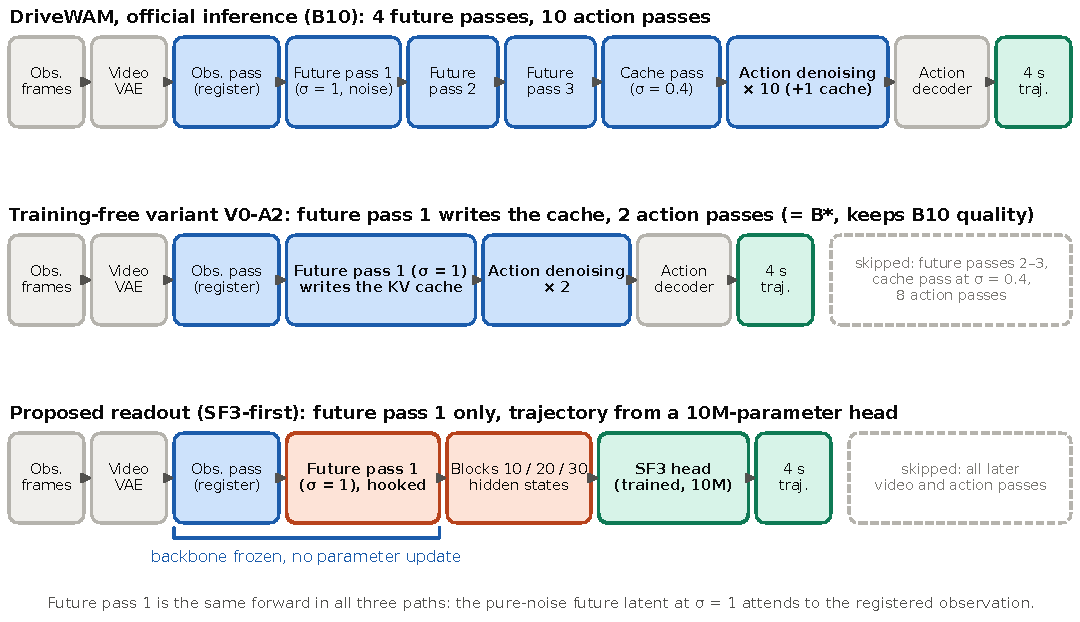
\includegraphics[width=\linewidth]{fig_overview.pdf}
\end{center}
\caption{Three ways to obtain a 4-second trajectory from DriveWAM. Top: official inference (B10) with four future passes and ten action-denoising passes. Middle: the training-free variant \VA{0}{2}, which writes the first future pass into the cache and denoises the action in two passes. Bottom: the proposed readout, which stops after the first future pass and predicts the trajectory with a 10M-parameter head from the hidden states of blocks 10, 20 and 30. The backbone is never updated.}
\label{fig:overview}
\end{figure}

\begin{figure}[t]
\begin{center}
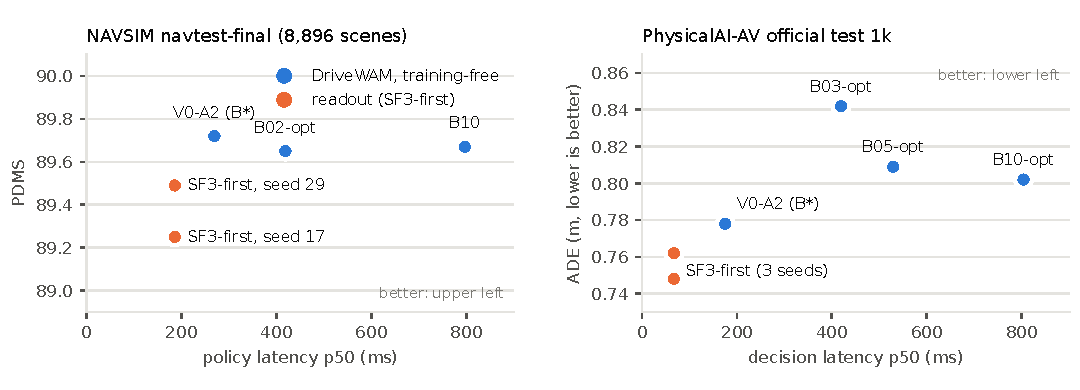
\includegraphics[width=\linewidth]{fig_tradeoff.pdf}
\end{center}
\caption{Quality versus median latency on the locked final sets (policy latency on NAVSIM, decision latency on PhysicalAI-AV; Section~\ref{sec:latency}). Blue: DriveWAM with the official schedule (B10) and training-free reduced-step variants, including \VA{0}{2}. Orange: the readout, one point per training seed. All latencies come from one session on an otherwise idle GPU.}
\label{fig:tradeoff}
\end{figure}

\section{Related work}
\label{sec:related}

\paragraph{Driving world models and world-action models.} Generative world models for driving such as GAIA-1 \citep{hu2023gaia} and Vista \citep{gao2024vista} learn to predict future frames; DriveWAM \citep{shi2026drivewam} generates video and actions as one token sequence under a joint flow-matching objective \citep{lipman2023flow}, with a frozen vision-language model supplying a guidance sentence per chunk and a selective KV memory bounding long rollouts. We use its public checkpoints and inference code unchanged.

\paragraph{Efficient action experts for WAMs.} Light-WAM \citep{li2026lightwam} pairs a compact video backbone with a state-fusion action expert that pools states from several backbone layers and predicts an action chunk in one forward pass. Two concurrent works named Faster-WAM argue that WAMs need only a shallow action expert reading all video layers \citep{ma2026fasterwam}, or that future representations should be computed once and reused throughout action denoising \citep{zhao2026fasterwam}. Our head adopts the multi-level state-fusion design of the Light-WAM expert, but the question differs: those works train or adapt the backbone together with the expert, whereas we keep a public driving WAM frozen and replace its own action generator. The result isolates what the pretrained world representation already contains and at which phase of the rollout it becomes available.

\paragraph{Diffusion features as representations.} Intermediate activations of image diffusion models carry semantic and geometric information \citep{xiang2023diffusionfeatures,tang2023dift}. Video Prediction Policy \citep{hu2025vpp} trains a robot policy on features from a single denoising pass of a video diffusion model, motivated by the idea that such features encode predicted dynamics. Our \first{} phase is the driving analogue inside a WAM, and the \current{}/\first{}/\terminal{} comparison tests the premise directly.

\paragraph{Training-free acceleration and few-step generation.} Feature caching across denoising steps \citep{ma2024deepcache}, reduced-step samplers, consistency models \citep{song2023consistency} and their policy variants \citep{prasad2024consistencypolicy}, and truncated diffusion planners \citep{liao2025diffusiondrive} attack the latency of diffusion inference from the generator side. Our training-free grid is the simplest member of this family: it changes only two step counts of the official sampler. A one-step distillation of DriveWAM's action generator would be a natural learned baseline and is left for future work.

\paragraph{Open-loop evaluation and the ego-state shortcut.} Open-loop driving metrics can be matched by models that use little more than the ego state \citep{zhai2023admlp,li2024egostatus}. We therefore report ego-only heads on both benchmarks, and on PhysicalAI-AV we measure how much of the readout's accuracy the ego state alone explains (Section~\ref{sec:where}).

\section{DriveWAM inference and the readout phases}
\label{sec:background}

DriveWAM is built on the Wan2.2-TI2V-5B video diffusion transformer (30 blocks, hidden size 3072), extended with action tokens and an action decoder; the full model has 6.24B parameters. One decision proceeds in three stages (Figure~\ref{fig:phases}).
\begin{enumerate}
\item \textbf{Observation pass.} The observed frames are encoded by a video VAE and registered in the KV cache, together with the past actions.
\item \textbf{Future passes.} A future video latent is initialized with Gaussian noise and denoised in three transformer passes at noise levels $\sigma = 1$, $0.8$ and $0.6$ (before the sampler's timestep shift); a fourth pass at $\sigma = 0.4$ does not update the latent but writes its keys and values into the cache for the action passes. DriveWAM stops the video denoising at 60\% of the schedule. We call these \emph{future passes 1 to 3} and the \emph{cache pass}.
\item \textbf{Action passes.} The action chunk (8 poses at 2 Hz on NAVSIM, 40 steps at 10 Hz on PhysicalAI-AV) is initialized with Gaussian noise and denoised in ten passes of the same transformer, which attend to the cached video and observation tokens; an eleventh pass writes the result into the cache, and a small decoder maps the action tokens to a trajectory. This is the official setting, \textbf{B10}.
\end{enumerate}
Guidance sentences from a frozen vision-language model and the ego state condition every pass. In the continuous PhysicalAI-AV setting the decision is repeated chunk by chunk with teacher forcing: after each chunk the predicted trajectory is discarded, and the recorded frame and actions are registered into memory in two passes before the next chunk (Figure~\ref{fig:pai}).

\paragraph{Reduced-step variants.} Both step counts can be changed without retraining. We write \VA{$v$}{$k$} for the variant with $v$ future-denoising steps and $k$ action-denoising steps that skips the final action cache pass, whose omission does not change the output. The official schedule is $v = 3$; with $v = 0$ the future schedule degenerates to the single pass at $\sigma = 1$, so the pure-noise latent is passed once and the keys and values of that pass are written into the cache. The variants with $v = 3$ are also written B10-opt, B05-opt, B03-opt, B02-opt and B01-opt. Table~\ref{tab:forwards} counts the backbone forwards.

\begin{table}[t]
\caption{Backbone forwards per decision (after the observation pass) and per PhysicalAI-AV clip (five chunks, including the 12 registration forwards). B10 includes the final action cache pass; the opt variants and the grid skip it.}
\label{tab:forwards}
\begin{center}
\small
\begin{tabular}{lcccc}
\toprule
Variant & future passes & action passes & per decision & per PhysicalAI-AV clip \\
\midrule
B10 (official) & 4 & 10 + 1 & 15 & 87 \\
B02-opt (\VA{3}{2}) & 4 & 2 & 6 & 42 \\
\VA{0}{2} & 1 & 2 & 3 & 27 \\
Readout (SF3-\first{}) & 1 & 0 (head) & 1 & 17 \\
\bottomrule
\end{tabular}
\end{center}
\end{table}

\paragraph{Readout phases.} Forward hooks read the outputs of transformer blocks 10, 20 and 30 (0-based 9, 19, 29) without altering them; each tap is a set of 112 video tokens of width 3072 on both benchmarks. The same tap can be read at three phases of the rollout:
\begin{itemize}
\item \current{}: during the observation pass; the backbone has registered the observed frames and has not processed any future latent.
\item \first{}: during future pass 1; the future tokens are pure noise that attends once to the observation cache.
\item \terminal{}: during the cache pass, after all updates of the future latent; this requires the full future generation.
\end{itemize}
The readout reads \first{} and exits immediately after that pass: the KV cache is released, and neither the remaining future passes nor any action pass is executed. Future pass 1 is the same forward in B10, in \VA{0}{2} and in the readout; the three paths differ only in what happens afterwards.

\begin{figure}[t]
\begin{center}
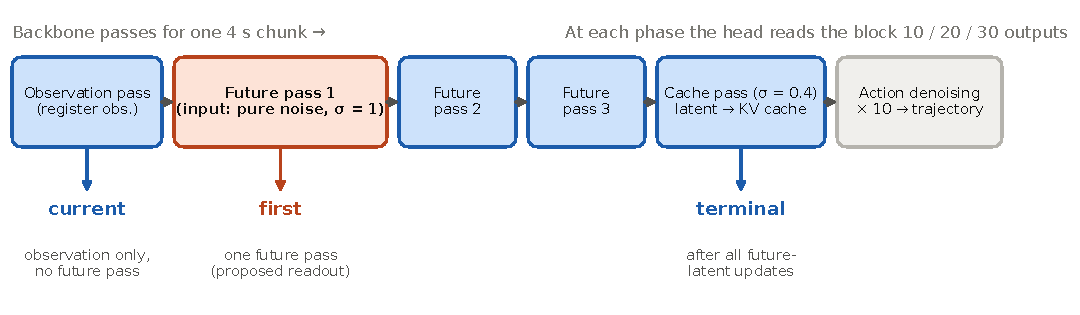
\includegraphics[width=\linewidth]{fig_phases.pdf}
\end{center}
\caption{The three readout phases for one 4-second chunk. The same head is trained separately for each phase; the readout uses \first{}. The variants with $v = 0$ run only the orange pass, with its outputs written into the cache.}
\label{fig:phases}
\end{figure}

\section{The readout head}
\label{sec:head}

The head, SF3, adopts the multi-level state-fusion design of the Light-WAM action expert \citep{li2026lightwam}: learned queries per tapped block, a fusion MLP and per-step decoding (Appendix~\ref{app:impl}, Figure~\ref{fig:sf3}). It differs in what it is attached to and what it predicts. It is trained alone on the frozen DriveWAM backbone, reads the backbone during future pass 1, takes the ego state as input, and predicts a normalized displacement and heading per step. Each tapped block is pooled by 16 learned queries into a 512-d state; the three states and a 128-d ego code are fused by an MLP into a driving state, from which a shared decoder with a learned time embedding predicts $(\Delta x, \Delta y, \Delta\theta)$ for each of the $K$ output steps ($K = 8$ on NAVSIM, $K = 40$ on PhysicalAI-AV). A cumulative sum gives poses. The head has 9.98M trainable parameters, 0.16\% of the backbone. The ego input is the driving command, four past poses, velocity and acceleration on NAVSIM (20-d), and velocity, acceleration and curvature on PhysicalAI-AV (5-d).

\paragraph{Training.} The loss is a Huber loss on positions plus $0.2\,(1 - \cos\Delta\theta)$ plus $0.1$ times a Huber loss on the normalized deltas. Every head is trained for 40 epochs with AdamW (learning rate $3 \times 10^{-4}$, weight decay 0.01, batch 32, 5\% warm-up, cosine decay) and evaluated at the last checkpoint, with no checkpoint selection on any evaluation set and batch-1 prediction as in deployment. Hidden states are cached once per phase and training set; the online policy (backbone with hooks plus head) reproduces the predictions made from cached states bitwise (Appendix~\ref{app:verification}). On PhysicalAI-AV the recorded actions are displacements in the clip-start frame. The head predicts in the chunk-start vehicle frame, and the prediction is rotated into the data frame with the heading accumulated from the already registered recorded actions; every method receives this information through memory. This choice was fixed before results were read and is decisive (Section~\ref{sec:needs}).

\paragraph{Controls.} An \emph{ego-only} head is the same architecture without the block poolers, so it predicts from the ego state alone. A \emph{constant-velocity} predictor and, on NAVSIM, single-level and flat-MLP heads serve as further references (Appendix~\ref{app:navsim-dev}).

\section{Experimental design}
\label{sec:setup}

\begin{table}[t]
\caption{Benchmarks, splits, references and the acceptance margins fixed in advance. ``CI'' is the 95\% bootstrap confidence interval of the paired difference. p50 is the median latency as defined in Section~\ref{sec:latency}.}
\label{tab:criteria}
\begin{center}
\small
\begin{tabular}{p{2.2cm}p{5.2cm}p{6.0cm}}
\toprule
 & NAVSIM v1.1 & PhysicalAI-AV \\
\midrule
Data & OpenScene revision \texttt{a76f840b} & NVIDIA revision \texttt{33f9bf44}, front camera; 23,994 of 24,000 clips processed \\
Unit & one scene $\rightarrow$ one 4-s trajectory (8 poses, 2 Hz) & one clip (21 frames at 1 fps) $\rightarrow$ 5 consecutive 4-s chunks (40 steps, 10 Hz), teacher forcing \\
Head-train & navtrain: 4k $\rightarrow$ 20k $\rightarrow$ 92,599 scenes (1,072 logs) & DriveWAM public train 4k $\subset$ 20k clips (all 5 chunks per clip) \\
Dev & navtest-dev: 34 logs, 3,250 scenes (split by log) & 1,000 validation clips (614 recordings); guidance sentences regenerated with the DriveWAM pipeline (Qwen3-VL-8B, \citealp{bai2025qwen3vl}; 27.8 words on average vs.\ 28.0 in the official prompts) \\
Final (locked, one run) & navtest-final: 102 logs, 8,896 scenes & official test 1k (480 recordings, public guidance sentences) \\
Metrics & official PDM score (PDMS) and its terms (NC, DAC, EP), ADE at 4 s & official ADE / FDE, chunk-level FDE $>$ 2 m rate \\
Reference & B10 (official inference) & B10-opt (official steps, no final action cache pass) \\
\Bstar{} rule (dev) & PDMS CI lower bound $\ge -2.0$ vs.\ B10; mean NC and DAC degradation $\le 0.5$; fastest such variant & ADE CI upper bound $\le +0.05$ m and FDE CI upper bound $\le +0.15$ m vs.\ B10-opt; fastest such variant \\
Readout margins & PDMS CI lower bound $\ge -2.0$ vs.\ B10 and \Bstar{}; NC/DAC degradation $\le 0.5$; p50 $\le 0.8 \times$ \Bstar{}; every seed & ADE CI upper $\le +0.05$ m and FDE CI upper $\le +0.15$ m vs.\ B10-opt and \Bstar{}; FDE $>$ 2 m rate increase $\le 1$ pp vs.\ B10-opt; p50 $\le 0.8 \times$ \Bstar{}; no p95 regression; every seed \\
Training seeds & 17, 29 & 17, 29, 43 \\
\bottomrule
\end{tabular}
\end{center}
\end{table}

\subsection{Benchmarks and splits}
\label{sec:benchmarks}

Table~\ref{tab:criteria} summarizes both benchmarks. On NAVSIM, a scene is scored by the official v1.1 scorer with the PDM score (PDMS), which combines no-collision (NC), drivable-area compliance (DAC), ego progress (EP), time-to-collision and comfort terms computed in a non-reactive simulation. On PhysicalAI-AV (Figure~\ref{fig:pai}) a clip yields five chunks; the official average and final displacement errors (ADE, FDE) reset to the recorded position at every chunk. Both evaluations are open-loop.

\paragraph{Why NAVSIM is split within navtest.} The public NAVSIM checkpoint was trained on navtrain, and it has memorized it: on a held-out navtrain subset B10 reaches 93.12 PDMS with an ADE of 0.076 m at 4 s, whereas on unseen navtest scenes it scores 90.93 PDMS with an ADE of 0.598 m, eight times larger (Appendix~\ref{app:navsim-dev}, Table~\ref{tab:memo}). A head trained and evaluated on navtrain states would learn a scene-to-trajectory shortcut; a classification head with 256 k-means anchors did exactly that, reaching 100\% training and 18.8\% validation accuracy. All development decisions were therefore moved to unseen scenes: navtest (136 logs) was shuffled with a fixed seed and split by log into a development part (34 logs, 3,250 scenes) and a final part (102 logs, 8,896 scenes). Head training still uses navtrain, where the backbone's states are those of memorized scenes; this is a limitation we return to in Section~\ref{sec:limitations}. Our B10 reproduction over all of navtest gives 90.01 PDMS, consistent with the 90.1 reported for the public checkpoint.

\paragraph{PhysicalAI-AV.} The development set is 1,000 random validation clips with guidance sentences regenerated by the DriveWAM pipeline, because the official validation prompts are not public; the final set is the official 1,000-clip test split with its public prompts. The route command inside each guidance sentence (go straight, turn left, turn right) is derived by the DriveWAM preprocessing from the recorded future ego pose, in the same way as the NAVSIM driving command; every method receives it. Our B10 reproduction on the test split gives ADE 0.802 m and FDE 2.384 m (the DriveWAM paper reports 0.83 and 2.47).

\begin{figure}[t]
\begin{center}
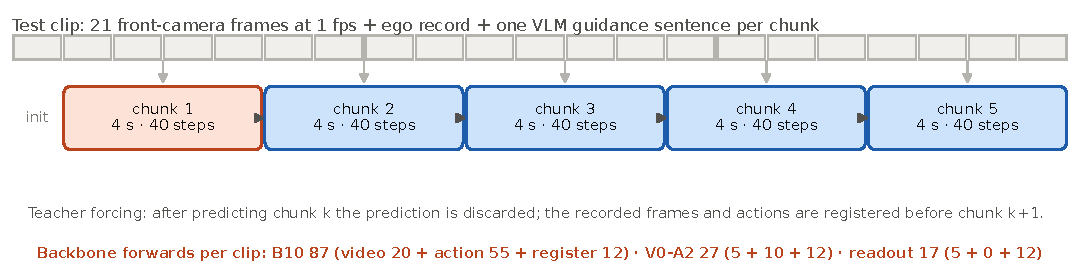
\includegraphics[width=\linewidth]{fig_pai.pdf}
\end{center}
\caption{PhysicalAI-AV evaluation unit. A 21-frame clip yields five 4-second chunks that are predicted with teacher forcing. The forward counts of B10 and of the readout were verified by instrumentation; that of \VA{0}{2} follows from Table~\ref{tab:forwards}.}
\label{fig:pai}
\end{figure}

\subsection{References and the training-free grid}
\label{sec:baselines}

The reference is the official DriveWAM inference, B10, timed as released on NAVSIM and without the final action cache pass (B10-opt) on PhysicalAI-AV, where that pass is never needed for the compared quantity. The reduced-step variants \VA{$v$}{$k$} with $v \in \{0,1,2,3\}$ and $k \in \{1,2,3,5\}$, together with B10-opt, form a grid of 17 training-free candidates; $k = 10$ with $v < 3$ was not run because such variants cannot be faster than the candidates with $k \le 5$ at the same $v$. All variants use the same noise as the official run (one fixed noise seed per scene on NAVSIM, noise seed 0 per clip on PhysicalAI-AV), and the action variants of one $v$ are computed from a single shared rollout; we verified on the first scenes and clips of every shard that the shared rollout reproduces separate runs bitwise. \textbf{\Bstar{}} is the fastest candidate that satisfies the \Bstar{} rule of Table~\ref{tab:criteria} on the development set; it represents the alternative ``just use fewer steps'' and is the reference the readout must beat on latency while matching on quality. The grid was run after a first version of this study had selected \Bstar{} among the $v = 3$ variants alone (B02-opt on NAVSIM, B03-opt on PhysicalAI-AV); both earlier choices are kept in the tables for comparison.

\subsection{Acceptance margins fixed in advance}
\label{sec:criteria}

To keep ourselves from choosing the comparison after the fact, the splits, the \Bstar{} rule, the head specification, the number of seeds and the margins within which we would call the readout acceptable were written down before results on the corresponding set were read, and the final sets were evaluated once per method. The margins (Table~\ref{tab:criteria}, ``Readout margins'') require quality within a fixed distance of both B10 and \Bstar{} and a median latency at most 0.8$\times$ that of \Bstar{}, for every training seed. We report them as one summary line per benchmark; the measurements themselves, with confidence intervals, are the result. Changes made during the work and the few places where we departed from the written plan are listed in Appendix~\ref{app:prereg}.

\subsection{Statistics}
\label{sec:stats}

Differences to a reference are reported with 95\% confidence intervals from a paired bootstrap with 2,000 resamples \citep{efron1994bootstrap}, resampling logs on NAVSIM and recordings (the dataset's chunk field) on PhysicalAI-AV, a cluster bootstrap, so that scenes and clips from the same drive are not treated as independent. Results are given per training seed; we do not average seeds.

\subsection{Latency}
\label{sec:latency}

The two benchmarks time different spans. On NAVSIM, \emph{policy latency} covers one call of the policy from the camera frame and ego state in host memory to the trajectory on the CPU: preprocessing, host-to-device transfer, VAE encoding, the observation pass and every later pass the method runs. The text embeddings of the four driving commands are precomputed. On PhysicalAI-AV, \emph{decision latency} runs from the end of registering the recorded history to the moment the action chunk is ready; VAE latents are computed once per clip and guidance embeddings are precomputed, so neither is timed, and the registration of the recorded chunk that follows is measured separately and reported as a per-chunk figure. The NAVSIM span therefore includes costs common to all methods, which makes its speed ratios conservative. All latencies in the main text come from one session per benchmark on an otherwise idle RTX A5000 (24 GB; host load average 1.2), the quiet-host session: on NAVSIM 256 final scenes, on PhysicalAI-AV 256 development clips, with the models alternated per scene or clip in three passes, 768 and 3,840 timed decisions per model, and a run-to-run variation of the median below 0.12\%. Earlier sessions on a shared host gave the same ratios and are listed in Appendix~\ref{app:impl}.

\subsection{Verification}
\label{sec:verification}

Before any result was read we verified bitwise that our re-implementation of the rollout equals the upstream inference, that the opt variants equal the raw implementation at equal step count, that hooks do not perturb outputs, that early-exit states equal the states captured during a full run, and that the online policy equals offline prediction from cached states; the full list is in Appendix~\ref{app:verification}. The NAVSIM inputs regenerated for the grid reproduce the stored B02-opt and readout trajectories within $10^{-5}$.

\section{Main results on the locked final sets}
\label{sec:main}

\begin{table}[t]
\caption{Locked final sets, each method evaluated once. NAVSIM: navtest-final (102 logs, 8,896 scenes), policy latency. PhysicalAI-AV: official test 1k (1,000 clips, 480 recordings), decision latency and, in parentheses, per-chunk latency including the registration of the recorded chunk. Ratios are to \VA{0}{2}. $\Delta$ rows give paired differences of the readout with 95\% CIs, for training seeds 17 / 29 (NAVSIM) and 17 / 29 / 43 (PhysicalAI-AV).}
\label{tab:final}
\begin{center}
\footnotesize
\setlength{\tabcolsep}{3.5pt}
\begin{tabular}{lcccccr}
\multicolumn{7}{l}{\textbf{NAVSIM navtest-final}} \\
\toprule
Model & PDMS & NC & DAC & EP & ADE (4 s) & p50 ms (ratio) \\
\midrule
B10 (official) & 89.67 & 98.12 & 97.97 & 83.83 & 0.564 m & 796.9 (2.96) \\
B02-opt (earlier \Bstar{}) & 89.65 & 98.15 & 97.93 & 83.81 & 0.564 m & 419.1 (1.55) \\
\VA{0}{2} (\Bstar{}) & 89.72 & 98.15 & 97.97 & 83.90 & 0.565 m & 269.6 (1.00) \\
Readout, seed 17 & 89.25 & 98.27 & 97.46 & 83.36 & 0.579 m & \textbf{186.3 (0.69)} \\
Readout, seed 29 & 89.49 & 98.30 & 97.62 & 83.52 & 0.577 m & \textbf{186.3 (0.69)} \\
\midrule
\multicolumn{7}{l}{$\Delta$PDMS, \VA{0}{2} $-$ B10: $+0.05\,[-0.11,+0.20]$.} \\
\multicolumn{7}{l}{$\Delta$PDMS, readout $-$ B10: seed 17 $-0.42\,[-0.76,-0.08]$; seed 29 $-0.17\,[-0.56,+0.27]$.} \\
\multicolumn{7}{l}{$\Delta$PDMS, readout $-$ \VA{0}{2}: seed 17 $-0.47\,[-0.81,-0.12]$; seed 29 $-0.22\,[-0.59,+0.23]$.} \\
\multicolumn{7}{l}{Scenes with a DAC violation: B10 181, \VA{0}{2} 181, readout 226 / 212.} \\
\bottomrule
\end{tabular}

\vspace{6pt}
\begin{tabular}{lcccr}
\multicolumn{5}{l}{\textbf{PhysicalAI-AV official test 1k}} \\
\toprule
Model & ADE (m) & FDE (m) & FDE $>$ 2 m (\%) & decision p50 / p95 ms (ratio); per chunk \\
\midrule
B10-opt (official steps) & 0.802 & 2.384 & 43.9 & 803.9 / 848.5 (4.58); 919.2 \\
B05-opt & 0.809 & 2.345 & 42.3 & 529.3 / 559.6 (3.02); 644.6 \\
B03-opt (earlier \Bstar{}) & 0.842 & 2.362 & 42.5 & 419.5 / 444.1 (2.39); 534.8 \\
\VA{0}{2} (\Bstar{}) & 0.778 & 2.170 & 39.3 & 175.4 / 185.5 (1.00); 290.6 \\
Readout, seed 17 & 0.750 & 2.244 & 41.4 & \textbf{67.4 / 71.7 (0.38); 183.2} \\
Readout, seed 29 & 0.748 & 2.244 & 41.0 & \textbf{67.4 / 71.7 (0.38); 183.2} \\
Readout, seed 43 & 0.762 & 2.287 & 42.1 & \textbf{67.4 / 71.7 (0.38); 183.2} \\
\midrule
\multicolumn{5}{l}{$\Delta$ADE vs.\ B10-opt: $-0.051\,[-0.070,-0.035]$ / $-0.054\,[-0.072,-0.036]$ / $-0.040\,[-0.057,-0.023]$} \\
\multicolumn{5}{l}{$\Delta$FDE vs.\ B10-opt: $-0.140\,[-0.198,-0.086]$ / $-0.141\,[-0.196,-0.088]$ / $-0.097\,[-0.152,-0.045]$} \\
\multicolumn{5}{l}{$\Delta$ADE vs.\ \VA{0}{2}: $-0.028\,[-0.045,-0.012]$ / $-0.030\,[-0.046,-0.014]$ / $-0.016\,[-0.032,-0.000]$} \\
\multicolumn{5}{l}{$\Delta$FDE vs.\ \VA{0}{2}: $+0.074\,[+0.021,+0.122]$ / $+0.073\,[+0.027,+0.117]$ / $+0.117\,[+0.068,+0.163]$} \\
\multicolumn{5}{l}{FDE $>$ 2 m rate vs.\ \VA{0}{2}: $+2.0$ / $+1.7$ / $+2.7$ pp} \\
\bottomrule
\end{tabular}
\end{center}
\end{table}

Table~\ref{tab:final} and Figure~\ref{fig:tradeoff} give the results on the locked final sets. Three observations hold on both benchmarks.

\paragraph{\VA{0}{2} keeps the official quality at a fraction of the cost.} The training-free variant with one future pass and two action passes scores 89.72 PDMS on NAVSIM against 89.67 for B10 ($+0.05\,[-0.11,+0.20]$), with the same number of drivable-area violations, and reaches 0.778 m ADE and 2.170 m FDE on PhysicalAI-AV against 0.802 and 2.384 m for B10-opt. Its median latency is 0.34$\times$ (NAVSIM) and 0.22$\times$ (PhysicalAI-AV) that of the official model. It replaces the earlier \Bstar{} choices B02-opt and B03-opt, which are 1.55$\times$ and 2.39$\times$ slower than \VA{0}{2} at equal or worse quality.

\paragraph{The readout is the fastest point, at a quality cost that depends on the metric.} With one backbone forward per decision, the readout's median latency is 186.3 ms on NAVSIM (0.69$\times$ \VA{0}{2}, 0.23$\times$ B10) and 67.4 ms on PhysicalAI-AV (0.38$\times$ \VA{0}{2}, 0.08$\times$ B10-opt). Including the registration of the recorded chunk, the per-chunk figure on PhysicalAI-AV is 183.2 ms against 290.6 ms for \VA{0}{2} and 919.2 ms for B10-opt. On NAVSIM the readout loses 0.42 and 0.17 PDMS to B10 and 0.47 and 0.22 PDMS to \VA{0}{2} for the two seeds; the loss sits in drivable-area compliance (226 and 212 violating scenes against 181) and ego progress, while the collision term improves by 0.15 to 0.17. On PhysicalAI-AV the readout has the lowest ADE of all methods for all three seeds ($-0.040$ to $-0.054$ m against B10-opt, $-0.016$ to $-0.030$ m against \VA{0}{2}, intervals below zero), a lower FDE than B10-opt ($-0.10$ to $-0.14$ m), and a higher FDE than \VA{0}{2} ($+0.07$ to $+0.12$ m, intervals above zero), with 1.7 to 2.7 percentage points more chunks whose endpoint error exceeds 2 m.

\paragraph{Against the margins fixed in advance.} On NAVSIM, seed 29 is within every margin; seed 17 exceeds the DAC margin against both references (degradation 0.506 against 0.5 allowed, i.e.\ one scene beyond the allowance). On PhysicalAI-AV, seeds 17 and 29 are within every margin; seed 43 exceeds the FDE margin against \VA{0}{2} ($+0.117$ m with an interval reaching 0.163 m against 0.15 allowed), while all three seeds are within the margins against B10-opt and against the earlier \Bstar{}. We therefore do not describe the readout as matching \VA{0}{2} in quality; it is a different point on the trade-off, 1.45$\times$ and 2.6$\times$ faster at the costs just listed. Development and final sets agree in sign and magnitude for every comparison (Appendices~\ref{app:navsim-dev} and \ref{app:pai-dev}).

\section{Where the action information is}
\label{sec:where}

\subsection{Readout phase}
\label{sec:phase}

The central comparison trains the same head on hidden states from the three phases of Section~\ref{sec:background} (Figure~\ref{fig:phase-results}, Table~\ref{tab:phase20k}). On NAVSIM with 4k training scenes, \first{} beats \current{} by $+3.40$ and $+3.28$ PDMS for the two seeds (intervals exclude zero), whereas \first{} versus \terminal{} is $-0.74\,[-2.11,+0.41]$ and $+0.61\,[+0.06,+1.16]$, changing sign across seeds. On PhysicalAI-AV with 4k training clips, \current{} costs $+0.106$ to $+0.123$ m ADE and $+0.41$ to $+0.46$ m FDE relative to \first{} for three seeds, while \terminal{} differs by $+0.008$ to $+0.014$ m with intervals including zero. The phase effect survives the data scale that the readout actually uses: with 20k training clips, \current{} heads reach 0.860 to 0.868 m ADE against 0.757 to 0.767 m for \first{} heads, a difference of $+0.094$ to $+0.111$ m ADE and $+0.33$ to $+0.39$ m FDE with intervals above zero for every seed. One pass over a pure-noise future latent produces most of the action-relevant information the head can use; the remaining three passes, which turn the noise into a video prediction, add nothing measurable for readout.

\begin{figure}[t]
\begin{center}
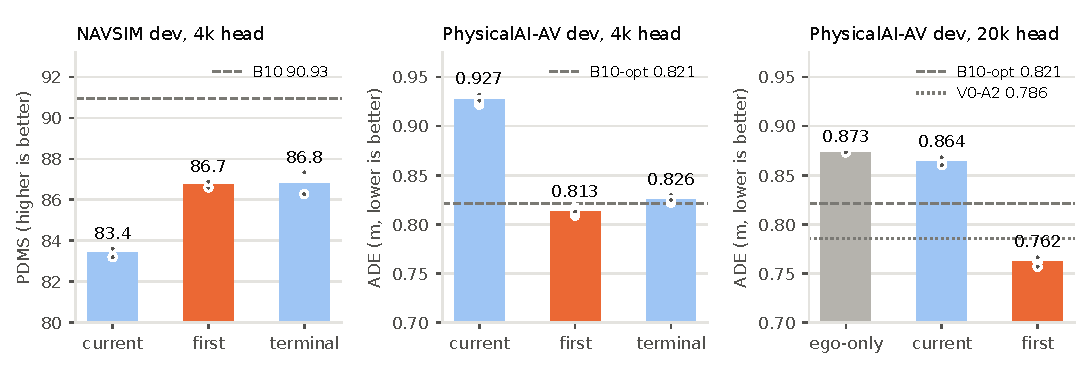
\includegraphics[width=\linewidth]{fig_phase_results.pdf}
\end{center}
\caption{Readout phase on the development sets. Bars are seed means, dots individual training seeds (two on NAVSIM, three on PhysicalAI-AV). Left and middle: 4k heads for all three phases. Right: 20k heads on PhysicalAI-AV with the ego-only head, which has no backbone input (the NAVSIM ego-only head scores 67.1 and 68.1 PDMS, and the constant-velocity predictor 1.900 m ADE on PhysicalAI-AV, both outside the plotted range).}
\label{fig:phase-results}
\end{figure}

\begin{table}[t]
\caption{PhysicalAI-AV development set, 20k heads, per training seed. Differences are paired, with 95\% CIs; FDE $>$ 2 m differences in percentage points.}
\label{tab:phase20k}
\begin{center}
\footnotesize
\setlength{\tabcolsep}{2.5pt}
\begin{tabular}{lccccc}
\toprule
Seed & \first{} ADE / FDE & \current{} ADE / FDE & ego-only ADE / FDE & $\Delta$ADE \current{} $-$ \first{} & $\Delta$ADE ego-only $-$ \first{} \\
\midrule
17 & 0.762 / 2.296 & 0.865 / 2.649 & 0.873 / 2.793 & $+0.103\,[+0.083,+0.123]$ & $+0.112\,[+0.089,+0.135]$ \\
29 & 0.757 / 2.284 & 0.868 / 2.676 & 0.873 / 2.794 & $+0.111\,[+0.090,+0.132]$ & $+0.116\,[+0.094,+0.140]$ \\
43 & 0.767 / 2.317 & 0.860 / 2.651 & 0.873 / 2.793 & $+0.094\,[+0.074,+0.113]$ & $+0.107\,[+0.084,+0.130]$ \\
\midrule
\multicolumn{6}{l}{$\Delta$FDE \current{} $-$ \first{}: $+0.35$ / $+0.39$ / $+0.33$ m; ego-only $-$ \first{}: $+0.50$ / $+0.51$ / $+0.48$ m (all CIs $>$ 0).} \\
\multicolumn{6}{l}{References on this set: B10-opt 0.821 / 2.452; \VA{0}{2} 0.786 / 2.194; constant velocity 1.900 / 5.332.} \\
\bottomrule
\end{tabular}
\end{center}
\end{table}

\subsection{The observation pass adds little to the ego state}
\label{sec:egoonly}

Open-loop driving metrics are known to be partly predictable from the ego state alone \citep{zhai2023admlp,li2024egostatus}, so the size of the backbone's contribution matters. On PhysicalAI-AV the ego-only head, trained on the same 20k clips with the same chunk-frame output, reaches 0.873 m ADE for all three seeds, 1.03 m better than constant velocity. The \current{} heads improve on it by only 0.005 to 0.013 m. The \first{} heads improve on it by 0.107 to 0.116 m ADE and 0.48 to 0.51 m FDE. Almost everything the frozen backbone contributes to the readout therefore appears in the first future pass, not in the observation pass. On NAVSIM the ego-only head scores 67.1 and 68.1 PDMS against 83.2 and 83.6 for \current{} and 86.6 and 86.9 for \first{} with 4k training scenes, so the observation pass is worth more there, but the first future pass still adds 3.3 PDMS on top of it.

\subsection{State-swap control}
\label{sec:swap}

The pilot study on the navtrain head-validation subset included a control in which a scene's hidden states were replaced by those of a different scene with a similar ego state. Every head collapsed from 76 to 87 PDMS to 35 to 41 PDMS, below the ego-only head (63.5 on that subset), which shows that the heads read scene-specific information from the hidden states rather than reconstructing the trajectory from the ego input.

\subsection{Sensitivity to the first-pass noise}
\label{sec:noise}

The \first{} states depend on the Gaussian noise that initializes the future latent. All heads were trained and, in the main results, evaluated with the noise of the official run (one fixed noise seed per scene or clip), so the readout is deterministic for that noise but not in general. Table~\ref{tab:noise} evaluates the trained heads on states computed with two further noise seeds, without retraining, and compares with DriveWAM under the same seeds. On NAVSIM the readout's PDMS changes by at most 0.19, its trajectories move by 0.14 m RMS between seeds, the same as B10's 0.13 m, and its ranking relative to B10 is unchanged. On PhysicalAI-AV the readout's ADE rises by 0.045 to 0.067 m on the other seeds and B10-opt's by 0.048 to 0.061 m on the same seeds; the readout's trajectories move by 0.93 to 1.01 m RMS between seeds against 1.14 to 1.36 m for B10-opt. The readout is therefore no more sensitive to the first-pass noise than the generator it replaces, and at every matched seed it stays 0.06 m ADE ahead of B10-opt (0.762 vs.\ 0.821 m, 0.807 vs.\ 0.869 m, 0.818 vs.\ 0.882 m for seed 17), even though the head never saw states from those seeds in training. Whether training on several noise seeds reduces the remaining sensitivity is an open question; we did not test it.

\begin{table}[t]
\caption{Sensitivity to the noise of future pass 1 on the development sets. Heads are the trained readouts (NAVSIM 92.6k, PhysicalAI-AV 20k), evaluated on states from noise seeds $g$ without retraining; $g = 0$ is the official noise used everywhere else. RMS is the mean root-mean-square displacement between the trajectories of seed $g$ and seed 0 on the same scenes or clips.}
\label{tab:noise}
\begin{center}
\footnotesize
\setlength{\tabcolsep}{4pt}
\begin{tabular}{llcccc}
\toprule
Benchmark & Model & $g = 0$ & $g = 1$ & $g = 2$ & RMS vs.\ $g = 0$ (m) \\
\midrule
NAVSIM (PDMS) & B10 & 90.93 & 91.21 & 91.20 & 0.137 / 0.132 \\
 & readout, seed 17 & 90.43 & 90.40 & 90.40 & 0.141 / 0.140 \\
 & readout, seed 29 & 90.58 & 90.47 & 90.39 & 0.146 / 0.142 \\
\midrule
PhysicalAI-AV (ADE, m) & B10-opt & 0.821 & 0.869 & 0.882 & 1.138 / 1.358 \\
 & readout, seed 17 & 0.762 & 0.807 & 0.818 & 0.925 / 0.951 \\
 & readout, seed 29 & 0.757 & 0.809 & 0.812 & 0.948 / 0.962 \\
 & readout, seed 43 & 0.767 & 0.817 & 0.834 & 0.991 / 1.013 \\
\bottomrule
\end{tabular}
\end{center}
\end{table}

\subsection{A possible confound: the guidance sentence}
\label{sec:guidance-confound}

On PhysicalAI-AV the \first{} pass is conditioned on the guidance sentence of the upcoming chunk, while the \current{} states come from the registration pass that used the previous chunk's sentence. The diagnostic of Section~\ref{sec:needs} bounds this effect: replacing the per-chunk sentence by a fixed default costs the \first{} head $+0.034$ to $+0.045$ m ADE, about one third of the \current{}--\first{} gap. A \first{} head without guidance (0.851 to 0.854 m) is still 0.07 m better than a \current{} head with guidance (0.922 to 0.932 m). The guidance explains part of the phase effect, not most of it.

\section{How much of the future the action generator needs}
\label{sec:howmuch}

If the readout can act from the first future pass, DriveWAM's own action generator might not need the denoised future either. The training-free grid of Section~\ref{sec:baselines} tests this directly (Figure~\ref{fig:grid}; full tables with confidence intervals in Appendix~\ref{app:grid}).

\begin{figure}[t]
\begin{center}
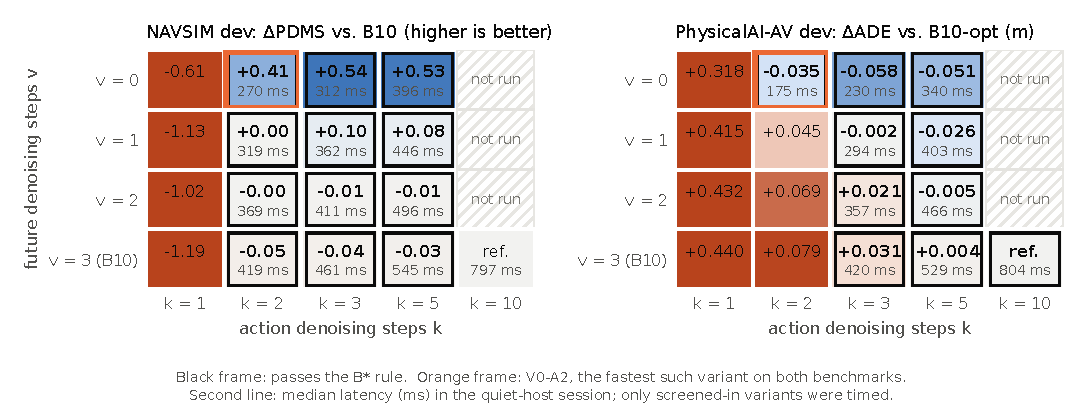
\includegraphics[width=\linewidth]{fig_grid.pdf}
\end{center}
\caption{Training-free grid on the development sets: $v$ future-denoising steps, $k$ action-denoising steps. Cells show the paired difference to the official schedule ($v = 3$, $k = 10$) and, where the variant passes the \Bstar{} rule, its median latency from the quiet-host session. Black frames mark variants that pass the \Bstar{} rule; the orange frame marks \VA{0}{2}, the fastest such variant on both benchmarks. Blue is better than the official schedule, red is worse.}
\label{fig:grid}
\end{figure}

\paragraph{Fewer future steps never hurt, and often help.} At every action step count $k \ge 2$, moving from the official $v = 3$ to $v = 0$ leaves NAVSIM PDMS unchanged or raises it, and lowers PhysicalAI-AV ADE. With $k = 3$, for instance, the paired difference to the official schedule goes from $-0.04$ ($v = 3$) to $-0.01$, $+0.10$ and $+0.54\,[+0.23,+0.86]$ PDMS ($v = 2, 1, 0$) on NAVSIM, and from $+0.031$ to $+0.021$, $-0.002$ and $-0.058\,[-0.069,-0.047]$ m ADE on PhysicalAI-AV. The trend is monotone in $v$ for every $k \ge 2$ on both benchmarks. The $v = 0$ variants with $k \ge 2$ are the best cells of each grid: $+0.41$ to $+0.54$ PDMS on NAVSIM and $-0.035$ to $-0.058$ m ADE with $-0.16$ to $-0.26$ m FDE on PhysicalAI-AV, all with intervals excluding zero. A single action pass is not enough at any $v$ ($-0.6$ to $-1.2$ PDMS; $+0.32$ to $+0.44$ m ADE), so two action passes are the floor for the native action generator.

\paragraph{\VA{0}{2} on the final sets.} The fastest variant that passes the \Bstar{} rule is \VA{0}{2} on both benchmarks (269.6 ms and 175.4 ms). Evaluated once on the locked final sets it confirms the development result: $+0.05$ PDMS against B10 on NAVSIM with an interval containing zero, and $-0.024$ m ADE, $-0.214$ m FDE against B10-opt on PhysicalAI-AV (Table~\ref{tab:final}). This is, to our knowledge, the simplest way to make DriveWAM 3.0$\times$ (NAVSIM) and 4.6$\times$ (PhysicalAI-AV) faster: set the future denoising to zero steps and the action denoising to two.

\paragraph{Interpretation.} With $v = 0$ the action passes attend to keys and values computed from a pure-noise future latent at $\sigma = 1$, that is, to the same forward that the readout reads. The grid therefore says about the action generator what Section~\ref{sec:where} says about the head: the backbone's first pass over the noisy future, conditioned on the registered observation, already carries what the action generation uses, and the video prediction that the later passes produce is not consumed by it. We can only speculate why more denoising slightly hurts. One reading is that a partially denoised future commits to one sample of a multimodal future, which the action generator then follows, whereas the $\sigma = 1$ pass is closer to an average over futures; mean-error metrics reward the latter (Section~\ref{sec:meaning}). We have not tested this reading.

\paragraph{The readout against \VA{0}{2}.} The readout removes the two remaining action passes and the action decoder and replaces them with the head. On NAVSIM this saves 83 ms of 270 (0.69$\times$) and costs 0.2 to 0.5 PDMS; on PhysicalAI-AV it saves 108 ms of 175 (0.38$\times$), lowers ADE by 0.02 to 0.03 m, and raises FDE by 0.07 to 0.12 m. Which of the two is preferable depends on the latency budget and on whether endpoint error matters more than mean error.

\section{What the readout needs}
\label{sec:needs}

\paragraph{Head-training scale.} With 4k head-training scenes every NAVSIM head lost 3.6 to 7.7 PDMS to B10, mostly through DAC and EP; a failure analysis located the loss in about 4\% of scenes in which only the head left the drivable area, at high speed or in turns. Among the remedies we tried, an FP32 output layer had no effect and an anchor-classification head failed (Appendix~\ref{app:navsim-dev}); the decisive factor was data. Figure~\ref{fig:scale} shows that with the same SF3-\first{} architecture the gap to B10 on navtest-dev shrank from $-4.2$ to $-1.3$ to $-0.4$ PDMS as head-training scenes grew from 4k to 20k to 92,599, the entire navtrain head-training split. On PhysicalAI-AV the 4k heads match B10-opt in ADE ($-0.005$ to $-0.012$ m) but raise the chunk-level rate of FDE $>$ 2 m by 2.3 to 3.7 percentage points; the 20k heads lower ADE by 0.055 to 0.064 m and the rate by 1.2 to 1.6 points. The 2 m threshold sits near the median chunk FDE of B10-opt (1.69 m), so this rate measures the body of the error distribution rather than its tail. Had we stopped at the 4k pilots we would have concluded, wrongly, that the states of a frozen world model contain too little action information. Training one 20k head takes 1.5 GPU-hours on the A5000 once the states are cached.

\begin{figure}[t]
\begin{center}
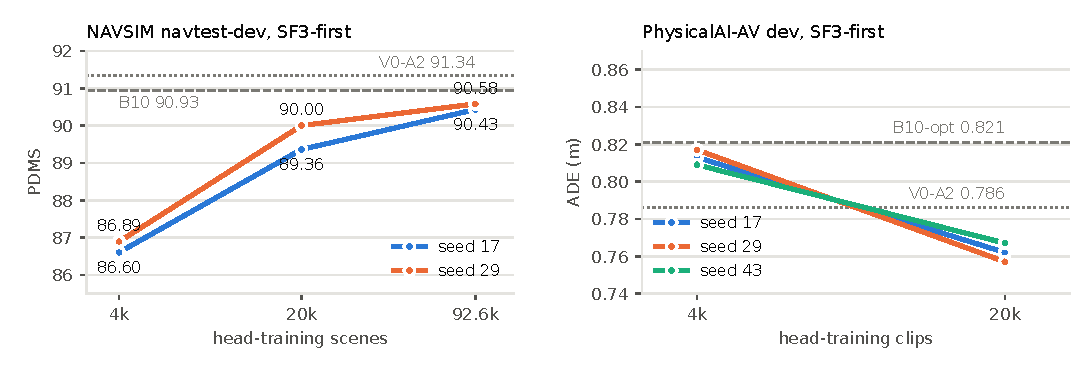
\includegraphics[width=\linewidth]{fig_scale.pdf}
\end{center}
\caption{Head-training scale with a fixed SF3-\first{} architecture on the development sets. Left: NAVSIM navtest-dev (seed means 86.7, 89.7 and 90.5 PDMS). Right: PhysicalAI-AV dev (seed means 0.813 and 0.762 m ADE). Dashed and dotted lines are B10 and \VA{0}{2} on the same sets.}
\label{fig:scale}
\end{figure}

\paragraph{Output frame.} On PhysicalAI-AV, predicting directly in the clip-start frame, our original specification, costs $+0.26$ m ADE; with it the readout would have been about 0.25 m worse than B10-opt. The rotation into the chunk-start vehicle frame was decided after inspecting the data convention and before results were read. We flag that this single choice decides whether the readout is competitive.

\paragraph{Memory and language guidance.} Table~\ref{tab:pai-diag} retrains the 4k head with three seeds under one change at a time. Removing the past-chunk memory (registering only the latest frame and zero actions) costs $+0.020$ to $+0.037$ m ADE; replacing the per-chunk guidance sentence by a fixed default costs $+0.034$ to $+0.045$ m. Both effects are significant and both are smaller than the phase effect of Section~\ref{sec:phase}.

\begin{table}[t]
\caption{PhysicalAI-AV development set, diagnostics with the 4k head (three seeds each). Differences are relative to the 4k \first{} head; ranges span the seeds.}
\label{tab:pai-diag}
\begin{center}
\small
\begin{tabular}{lccc}
\toprule
Setting & ADE (m) & $\Delta$ADE vs.\ \first{} & $\Delta$FDE vs.\ \first{} \\
\midrule
\first{} (reference) & 0.809--0.817 & -- & -- \\
\current{} (observation pass only) & 0.922--0.932 & $+0.106$ to $+0.123$ (all CIs $>$ 0) & $+0.41$ to $+0.46$ \\
\terminal{} (after all future passes) & 0.822--0.830 & $+0.008$ to $+0.014$ (CIs include 0) & $+0.02$ to $+0.04$ \\
no memory (latest frame, zero actions) & 0.837--0.846 & $+0.020$ to $+0.037$ (all CIs $>$ 0) & $+0.06$ to $+0.14$ \\
fixed prompt (no per-chunk guidance) & 0.851--0.854 & $+0.034$ to $+0.045$ (all CIs $>$ 0) & $+0.14$ to $+0.19$ \\
clip-frame output (original specification) & 1.070--1.085 & $+0.260$ to $+0.269$ (all CIs $>$ 0) & $+0.38$ to $+0.41$ \\
\bottomrule
\end{tabular}
\end{center}
\end{table}

\paragraph{Head architecture.} Multi-level pooling (SF3) versus a single wide level is directionally consistent on NAVSIM but significant in only one seed, and a flat MLP on pooled states is worse (Appendix~\ref{app:navsim-dev}, Table~\ref{tab:navsim-phases}). We leave the question of the best tapping depth open; the three-block head was fixed before the main runs and never tuned.

\section{What the accuracy numbers mean}
\label{sec:meaning}

\paragraph{Determinism control.} The readout is a deterministic regressor, while DriveWAM samples an action chunk from noise. The official PhysicalAI-AV protocol uses seed 0 for every clip, so a single seed moves the whole benchmark score in one direction. Table~\ref{tab:determinism} shows that B10-opt's development ADE ranges from 0.821 m (seed 0) to 0.930 m (seed 3), with a mean of 0.876 m over the four seeds, and that averaging the trajectories of $k$ seeds lowers it to 0.765 to 0.781 m. Against the four-sample mean the readout is on par in ADE ($-0.011$ to $-0.021$ m, two of three intervals include zero) and 0.08 to 0.12 m worse in FDE (intervals above zero). Most of the readout's accuracy advantage over the official single sample is therefore an effect of determinism on mean-error metrics; the official seed 0 was also the best of the four, so the comparison in Table~\ref{tab:final} is, if anything, conservative for the readout. The appropriate reading is that the readout reaches the ADE of a four-sample average of DriveWAM, but not its FDE, in one pass. The four-sample average itself needs four full rollouts and would be slower than B10-opt even if batched, which we did not measure.

\begin{table}[t]
\caption{Determinism control on the PhysicalAI-AV development set (post-hoc analysis). The official protocol uses seed 0 for all clips.}
\label{tab:determinism}
\begin{center}
\footnotesize
\setlength{\tabcolsep}{2pt}
\begin{tabular}{lccc}
\toprule
B10-opt prediction & ADE (m) & FDE (m) & FDE $>$ 2 m (\%) \\
\midrule
one sample, seed 0 (official) / 1 / 2 / 3 & 0.821 / 0.869 / 0.882 / 0.930 & 2.452 / 2.453 / 2.542 / 2.647 & 43.1 / 44.2 / 46.3 / 48.0 \\
mean of 2 / 3 / 4 samples & 0.781 / 0.765 / 0.777 & 2.250 / 2.179 / 2.200 & 39.0 / 38.7 / 39.5 \\
\midrule
readout, 20k, seeds 17 / 29 / 43 & 0.762 / 0.757 / 0.767 & 2.296 / 2.284 / 2.317 & 41.5 / 41.5 / 41.8 \\
\multicolumn{4}{l}{readout $-$ 4-sample mean (seeds 17 / 29 / 43):} \\
\multicolumn{4}{l}{\quad $\Delta$ADE $-0.016\,[-0.032,+0.001]$ / $-0.021\,[-0.037,-0.004]$ / $-0.011\,[-0.028,+0.006]$} \\
\multicolumn{4}{l}{\quad $\Delta$FDE $+0.096\,[+0.049,+0.148]$ / $+0.084\,[+0.037,+0.132]$ / $+0.117\,[+0.066,+0.167]$; FDE $>$ 2 m $+1.9$ to $+2.3$ pp} \\
\bottomrule
\end{tabular}
\end{center}
\end{table}

\paragraph{Why the two benchmarks disagree about the readout.} The readout is behind both references on NAVSIM and ahead of them in ADE on PhysicalAI-AV. We can only hypothesize about the cause. PDMS is a rule-based score in which a deterministic prediction has nothing to gain from averaging and in which an averaged trajectory at a fork can leave the drivable area, which is where the readout loses; ADE and FDE reward exactly such averaging. The continuous setting also supplies memory and guidance, which the diagnostics show the head uses. Sample counts were similar (92.6k scenes against about 100k chunks from 20k clips), although the chunks of one clip are correlated, so the data argument is not clean. We do not conclude that the readout works better on PhysicalAI-AV, only that the PhysicalAI-AV metrics favor deterministic prediction and the NAVSIM metric does not.

\paragraph{Residual losses.} The readout's residual losses are drivable-area compliance on NAVSIM and the 4-second endpoint on PhysicalAI-AV. Both are compatible with a regression head averaging over a multimodal future; we have not verified this cause. Multimodal or safety-oriented metrics and closed-loop evaluation are needed before any safety claim. The seed study of Section~\ref{sec:noise} adds one more fact: DriveWAM's own trajectories move by 0.13 m RMS between noise seeds on NAVSIM, far more than the readout's mean ADE gap to B10 (0.015 m), which suggests that the remaining PDMS gap comes from a small number of scenes, such as the 31 to 45 additional drivable-area violations, rather than from a uniform offset.

\paragraph{Evaluation practice.} Two observations apply beyond this paper. Public checkpoints may have memorized public training splits, so readout and probing studies should use unseen scenes and should be wary of classification heads. Single-seed protocols for stochastic policies can be lucky or unlucky; comparisons between a stochastic generator and a deterministic method should report several seeds or multi-sample averages, as in Tables~\ref{tab:noise} and \ref{tab:determinism}.

\section{Limitations}
\label{sec:limitations}

Our results concern one world model (DriveWAM) and two open-loop, non-reactive benchmarks; closed-loop behavior is untested. NAVSIM heads are trained on navtrain scenes that the backbone has memorized, so their training states are not those of unseen scenes, and we do not know how much this costs. Verdicts rest on two training seeds on NAVSIM and three on PhysicalAI-AV, and the readout is deterministic only for a fixed first-pass noise (Section~\ref{sec:noise}). The PhysicalAI-AV development set is a random validation subset while the official test set is VLM-curated; B10-opt's ADE was similar on both (0.821 against 0.802 m). The chunk-frame output rotation on PhysicalAI-AV decides the outcome. A deterministic head is favored by mean-error metrics. The grid varies only two step counts; a one-step distillation of the action generator, a second world model and a batched multi-sample baseline were not run. Latency is a ratio measured on one GPU, with different timed spans on the two benchmarks (Section~\ref{sec:latency}). The multi-level versus single-level hypothesis is significant in only one seed, and the NAVSIM final run was made although the development result had missed the DAC margin by one scene (Appendix~\ref{app:prereg}).

\section{Conclusion}
\label{sec:conclusion}

A frozen driving world-action model forms, during its first pass over a pure-noise future latent, a representation that both its own action generator and a 10M-parameter head can act on. Running only that pass makes DriveWAM 3.0$\times$ and 4.6$\times$ faster on two benchmarks with no quality loss, and reading the trajectory from it with the head makes it 4.3$\times$ and 11.9$\times$ faster at a quality cost of 0.2 to 0.5 PDMS on NAVSIM and of 0.07 to 0.12 m FDE on PhysicalAI-AV, where its ADE is the lowest of all methods. Completing the imagination does not improve the action; enough head-training labels are required to see this; and mean-error metrics flatter deterministic prediction. The training-free grid, the fixed-margin comparison and the documented evaluation pitfalls may be useful to others studying what world models already know about acting.

\subsubsection*{Broader Impact Statement}
This work reduces the inference cost of a driving policy evaluated in open loop. Faster inference could make world-action models more practical for deployment, but nothing here establishes closed-loop safety; the residual losses on drivable-area compliance and 4-second endpoints are exactly the terms a safety case would scrutinize. We caution against reading the open-loop accuracy numbers as evidence of safe driving.

\bibliography{../references}
\bibliographystyle{tmlr}

\appendix

\section{Protocol documents and recorded changes}
\label{app:prereg}

Each benchmark was run under a written protocol that fixed, before any prediction on the corresponding set was produced, the split rule and its file hash, the reference set and the \Bstar{} rule, the head architecture and training protocol, the number of seeds, the acceptance margins, the bootstrap procedure and the latency protocol. Changes made during the work were appended with a date before the affected results were read, and the locked final sets were evaluated once per method. The documents are provided, anonymized, as supplementary material. The points that matter for reading the results are the following.

\paragraph{NAVSIM.} navtest (136 logs) was shuffled with a fixed seed and split by log into 34 development logs and 102 final logs after the memorization of navtrain had been found. The pilot had selected checkpoints on an evaluation set; the protocol used for all reported heads fixes 40 epochs, the last checkpoint and two training seeds. Development predictions were first computed with batch 64 and recomputed with batch 1 after a BF16 output layer was found to change trajectories at the centimeter level with batch size (PDMS within $\pm 0.2$). The final run of the 92.6k head was made although the development result had missed the DAC margin by one scene; the decision was recorded before the run and the checkpoints were frozen by hash.

\paragraph{PhysicalAI-AV.} Ten changes were recorded before results, including: the development set was switched to 1,000 random validation clips because the upstream scene-tagging script exceeded the 24 GB GPU; each test clip yields five rather than four chunks, as verified by the parity check; the head is trained on all five chunks; the head-training size (4k or 20k) was chosen by the lower seed-averaged development ADE; and the output frame was changed to the chunk-start vehicle frame after inspecting the data convention. The determinism control and the matched-seed comparison are post-hoc analyses.

\paragraph{Follow-up experiments.} The training-free grid, the 20k \current{} and ego-only heads, the noise-seed study and the quiet-host latency session were specified in a follow-up document, written after an internal review of a first draft and before any of their results existed. It fixed the grid, the screening rule (the existing \Bstar{} rule), the latency protocol, the rule for re-selecting \Bstar{} and the interpretation rules for the phase and noise studies. Under that document, a changed \Bstar{} required one run of the new \Bstar{} on each final set and a re-evaluation of the readout against it; the readout's final predictions were not recomputed.

\section{Bitwise verification list}
\label{app:verification}

\begin{table}[H]
\caption{Verifications performed before the corresponding results were read.}
\begin{center}
\small
\begin{tabular}{p{7.5cm}p{3.8cm}p{3cm}}
\toprule
Check & Scope & Result \\
\midrule
Rollout re-implementation $=$ upstream inference (B10, B05) & NAVSIM pilot scenes; PhysicalAI-AV 3 final clips & bitwise equal \\
opt (skip final action cache pass) $=$ raw at equal step count & NAVSIM; PhysicalAI-AV 3 final + 32 dev clips & bitwise equal \\
Shared multi-variant rollout $=$ individual runs & PhysicalAI-AV 3 final clips; grid: 4 scenes or clips per shard & bitwise equal \\
Hooks do not perturb outputs; early-exit states $=$ states captured during a full run & NAVSIM; PhysicalAI-AV 3 final + 32 dev clips & bitwise equal \\
Readout metric path $=$ official metric code & 6 clips $\times$ 5 models & max.\ difference $7 \times 10^{-6}$ m \\
Memory-mapped training inputs $=$ stored states & train-4k sample & bitwise equal (identical epoch losses) \\
Online policy (backbone $+$ head) $=$ offline predictions from cached states & NAVSIM final; PhysicalAI-AV 128 clips, 640 chunks & bitwise equal \\
Vehicle-frame / clip-frame rotation round trip & training sample & max.\ error $2.4 \times 10^{-7}$ (normalized units) \\
Backbone forwards per clip & PhysicalAI-AV & B10 87, readout 17 \\
Our 1 fps frame store $=$ upstream video loader & 4 dev clips & bitwise equal \\
Regenerated NAVSIM inputs reproduce stored trajectories (B02-opt, readout) & first scenes of every shard & within $10^{-5}$ \\
\bottomrule
\end{tabular}
\end{center}
\end{table}

\section{Implementation details}
\label{app:impl}

\paragraph{Environment.} PyTorch 2.9.0 with CUDA 12.6, flash-attention 2.8.3, diffusers 0.36.0, transformers 4.55.2, two RTX A5000 (24 GB) GPUs. Upstream commits, model revisions and file hashes are pinned in a source-lock file released with the code. The official NAVSIM scorer runs in a separate CPU environment.

\paragraph{Head.} Figure~\ref{fig:sf3} shows the SF3 head. Taps at blocks 10/20/30; per block LayerNorm $\rightarrow$ Linear $3072 \rightarrow 512$ $\rightarrow$ 16 learned queries with 8-head attention $\rightarrow$ learned weighted sum over queries $\rightarrow$ LayerNorm; ego MLP to 128-d; fusion 1,664 $\rightarrow$ 512 with GELU, residual MLP 512 $\rightarrow$ 1024 $\rightarrow$ 512; decoder LayerNorm $\rightarrow$ 512 $\rightarrow$ 256 $\rightarrow$ 3 in FP32 with a learned time embedding per output step; 9.98M parameters. Targets are normalized with 1\%/99\% quantiles. AdamW, learning rate $3 \times 10^{-4}$, weight decay 0.01, batch 32, 40 epochs, 5\% linear warm-up then cosine decay, last checkpoint, seeds 17/29 (NAVSIM) and 17/29/43 (PhysicalAI-AV). Training one PhysicalAI-AV head takes 0.3 GPU-hours with 4k clips and 1.5 GPU-hours with 20k clips; the ego-only head takes 0.45 GPU-hours.

\begin{figure}[H]
\begin{center}
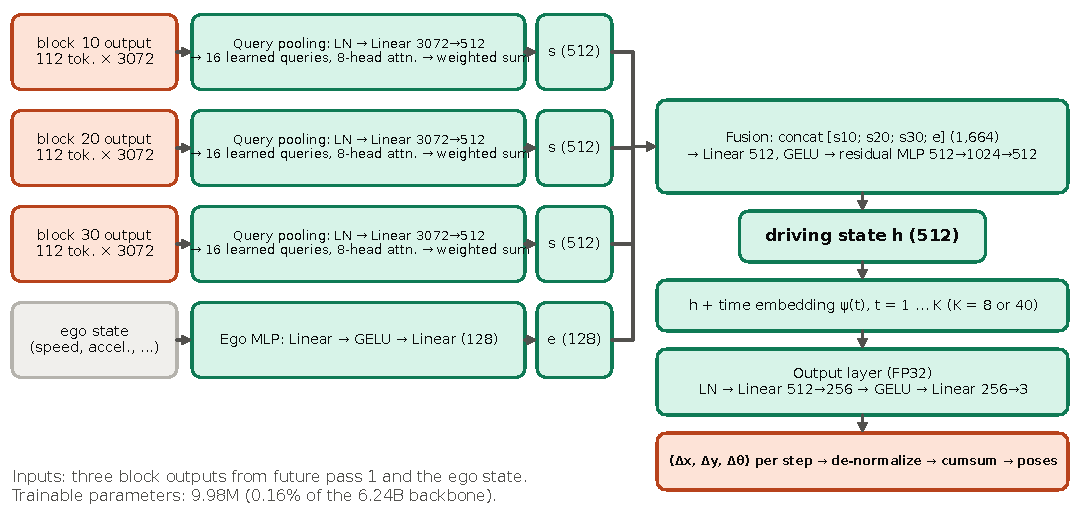
\includegraphics[width=0.95\linewidth]{fig_sf3.pdf}
\end{center}
\caption{SF3 head. Three tapped blocks are pooled with learned queries, fused with the ego state, and decoded step by step. Only the head is trained.}
\label{fig:sf3}
\end{figure}

\paragraph{Guidance sentences for the PhysicalAI-AV development set.} The official test prompts are public; for the validation clips we regenerated guidance sentences with the DriveWAM three-stage pipeline using Qwen3-VL-8B \citep{bai2025qwen3vl}. The sentences average 27.8 words against 28.0 in the official prompts. On torch 2.9 with cuDNN 9.10 the bf16 Conv3d patch embedding of the VLM took about 10 s per call; we replaced it with the mathematically identical linear operation (0.3 ms, same error relative to an FP32 reference). The upstream evaluator caches prompt embeddings on the GPU indefinitely; we clear the cache per clip (values identical).

\paragraph{Latency sessions.} The main-text latencies come from one session per benchmark on 2026-11-01 on an idle host (load average 1.2): NAVSIM 256 final scenes, 14 models alternated per scene, three passes, 768 timed calls per model, run-to-run variation of the median at most 0.11\%; PhysicalAI-AV 256 development clips on two GPUs, 11 models alternated per clip, three passes, 3,840 timed decisions per model. Earlier sessions on the same GPUs while other jobs ran (host load 12 to 60) gave readout medians of 189.0 ms (NAVSIM) and 70.9 ms (PhysicalAI-AV) and ratios to B02-opt and B03-opt of 0.449 and 0.163, against 0.445 and 0.161 in the quiet session; absolute times drifted by up to 30\% across days on the shared host, which is why only same-session ratios are used anywhere in this paper.

\section{Additional NAVSIM results}
\label{app:navsim-dev}

\begin{table}[H]
\caption{Backbone memorization on NAVSIM. ADE is the average displacement error of the 4-second trajectory.}
\label{tab:memo}
\begin{center}
\small
\begin{tabular}{lcc}
\toprule
Model & navtrain head-val (256 scenes) & navtest-dev (3,250 scenes, unseen) \\
 & PDMS / ADE & PDMS / ADE \\
\midrule
B10 & 93.12 / 0.076 m & 90.93 / 0.598 m \\
B02-opt & 92.75 / 0.077 m & 90.88 / 0.599 m \\
SF3-\terminal{}, 4k head (pilot protocol) & 86.72 / 0.317 m & 85.59 / 0.674 m \\
\bottomrule
\end{tabular}
\end{center}
\end{table}

\begin{table}[H]
\caption{NAVSIM navtest-dev, 4k-scene heads (40 epochs, last checkpoint, batch-1 prediction). $\Delta$ is the paired difference to B10 (PDMS 90.93) with its 95\% CI; the last column is the median latency relative to B02-opt in the session of that round.}
\label{tab:navsim-phases}
\begin{center}
\footnotesize
\setlength{\tabcolsep}{4pt}
\begin{tabular}{llccc}
\toprule
Head & Phase & PDMS seed 17 / 29 & $\Delta$ vs.\ B10, seed 17 / 29 & p50 / B02-opt \\
\midrule
SF3 & \terminal{} & 87.34 / 86.28 & $-3.59\,[-4.92,-2.42]$ / $-4.65\,[-6.42,-3.14]$ & 0.794 \\
SF3 & \first{}    & 86.60 / 86.89 & $-4.34\,[-6.17,-2.81]$ / $-4.04\,[-5.89,-2.50]$ & 0.467 \\
SF3 & \current{}  & 83.20 / 83.61 & $-7.73\,[-9.97,-5.86]$ / $-7.32\,[-9.43,-5.45]$ & 0.248 \\
SF1 (block 30) & \terminal{} & 85.38 / 84.79 & $-5.55$ / $-6.15$ & 0.794 \\
SF1-wide & \terminal{} & 83.64 / 85.04 & $-7.29$ / $-5.89$ & -- \\
Flat MLP & \terminal{} & 83.00 / 84.16 & $-7.94$ / $-6.77$ & 0.796 \\
Ego-only & -- & 67.07 / 68.10 & $-23.9$ / $-22.8$ & -- \\
\bottomrule
\end{tabular}
\end{center}
\end{table}

\begin{table}[H]
\caption{NAVSIM navtest-dev, remedies tried with the 4k heads and the effect of head-training scale. Differences are to B10 (90.93 PDMS).}
\begin{center}
\footnotesize
\setlength{\tabcolsep}{3pt}
\begin{tabular}{llccc}
\toprule
Train & Head / phase & PDMS 17 / 29 & $\Delta$ vs.\ B10 [95\% CI], seed 17 / 29 & DAC degr. \\
\midrule
4k & SF3 regression, FP32 output, \terminal{} & 86.58 / 87.04 & $-4.35$ / $-3.89$ & -- \\
4k & SF3 anchor head ($K$=256), \first{} & 57.85 / 59.08 & $-33.1$ / $-31.9$ & -- \\
20k & SF3 anchor head ($K$=256), \first{} & 79.53 / 78.96 & $-11.4$ / $-12.0$ & -- \\
20k & SF3 regression, \first{} & 89.36 / 90.00 & $-1.57\,[-2.62,-0.71]$ / $-0.94\,[-1.95,+0.00]$ & $-1.51$ / $-1.05$ \\
20k & SF3 regression, \terminal{} & 89.47 / 89.10 & $-1.46\,[-2.43,-0.57]$ / $-1.83\,[-3.00,-0.86]$ & $-1.54$ / $-1.72$ \\
92.6k & SF3 regression, \first{} & 90.43 / 90.58 & $-0.51\,[-1.12,+0.14]$ / $-0.36\,[-0.95,+0.28]$ & $-0.52$ / $-0.40$ \\
\bottomrule
\end{tabular}
\end{center}
\end{table}

The pilot on the navtrain head-validation subset included the state-swap control of Section~\ref{sec:swap}. A noise-seed study of B10 on 32 unseen scenes found a mean RMS spread of 6.0 cm between the trajectories of different seeds, against 3.5 cm on memorized navtrain scenes; the full-dev figures with two seeds are in Table~\ref{tab:noise}.

\section{Additional PhysicalAI-AV results}
\label{app:pai-dev}

\begin{table}[H]
\caption{PhysicalAI-AV development set, readout heads per seed (\first{} phase, vehicle-frame output). The \Bstar{} column refers to the earlier \Bstar{}, B03-opt.}
\begin{center}
\footnotesize
\setlength{\tabcolsep}{4pt}
\begin{tabular}{lcccccc}
\toprule
Head & ADE & FDE & $\Delta$ADE vs.\ B10-opt & $\Delta$ADE vs.\ B03-opt & FDE$>$2 m (pp vs.\ B10-opt) \\
\midrule
20k, seed 17 & 0.762 & 2.296 & $-0.059\,[-0.078,-0.040]$ & $-0.091\,[-0.109,-0.072]$ & $-1.58$ \\
20k, seed 29 & 0.757 & 2.284 & $-0.064\,[-0.082,-0.046]$ & $-0.095\,[-0.113,-0.078]$ & $-1.60$ \\
20k, seed 43 & 0.767 & 2.317 & $-0.055\,[-0.072,-0.037]$ & $-0.086\,[-0.103,-0.068]$ & $-1.24$ \\
4k, seed 17 & 0.813 & 2.445 & $-0.008\,[-0.026,+0.011]$ & $-0.039\,[-0.057,-0.021]$ & $+2.62$ \\
4k, seed 29 & 0.817 & 2.460 & $-0.005\,[-0.023,+0.013]$ & $-0.036\,[-0.054,-0.018]$ & $+3.72$ \\
4k, seed 43 & 0.809 & 2.421 & $-0.012\,[-0.031,+0.007]$ & $-0.043\,[-0.062,-0.024]$ & $+2.34$ \\
\bottomrule
\end{tabular}
\end{center}
\end{table}

Development and final results agree in ranking and magnitude: on the final set the 20k readout's differences to B10-opt are $-0.040$ to $-0.054$ m ADE (Table~\ref{tab:final}) against $-0.055$ to $-0.064$ m on the development set. The earlier reduced-step references on the final set are B05-opt 0.809 / 2.345 m, B02-opt 0.891 / 2.420 m and B01-opt 1.272 / 3.000 m (ADE / FDE).

\section{Training-free grid: full tables}
\label{app:grid}

\begin{table}[H]
\caption{NAVSIM navtest-dev (3,250 scenes): training-free variants against B10 (90.93 PDMS). Paired differences with 95\% CIs; NC and DAC are mean degradations (positive = worse). The \Bstar{} rule requires a PDMS CI lower bound $\ge -2.0$ and NC and DAC degradations $\le 0.5$. Latency: median policy latency in the quiet-host session, measured only for variants that pass the rule.}
\begin{center}
\footnotesize
\setlength{\tabcolsep}{4pt}
\begin{tabular}{lccrrcc}
\toprule
Variant & $v$ & $k$ & $\Delta$PDMS [95\% CI] & NC / DAC degr. & passes & p50 (ms) \\
\midrule
B05-opt & 3 & 5 & $-0.03\,[-0.20,+0.11]$ & 0.00 / 0.00 & yes & 545.2 \\
B03-opt & 3 & 3 & $-0.04\,[-0.23,+0.14]$ & 0.03 / $-$0.03 & yes & 461.2 \\
B02-opt & 3 & 2 & $-0.05\,[-0.25,+0.14]$ & 0.00 / 0.00 & yes & 419.1 \\
B01-opt & 3 & 1 & $-1.19\,[-1.96,-0.53]$ & 0.02 / 1.11 & no & -- \\
\VA{2}{5} & 2 & 5 & $-0.01\,[-0.18,+0.13]$ & $-$0.03 / 0.00 & yes & 495.7 \\
\VA{2}{3} & 2 & 3 & $-0.01\,[-0.20,+0.17]$ & 0.00 / $-$0.03 & yes & 411.4 \\
\VA{2}{2} & 2 & 2 & $-0.00\,[-0.21,+0.18]$ & $-$0.03 / $-$0.03 & yes & 369.3 \\
\VA{2}{1} & 2 & 1 & $-1.02\,[-1.78,-0.40]$ & $-$0.08 / 1.02 & no & -- \\
\VA{1}{5} & 1 & 5 & $+0.08\,[-0.09,+0.25]$ & $-$0.09 / $-$0.06 & yes & 445.6 \\
\VA{1}{3} & 1 & 3 & $+0.10\,[-0.12,+0.30]$ & $-$0.09 / $-$0.09 & yes & 361.5 \\
\VA{1}{2} & 1 & 2 & $+0.00\,[-0.21,+0.19]$ & $-$0.09 / 0.00 & yes & 319.4 \\
\VA{1}{1} & 1 & 1 & $-1.13\,[-1.95,-0.41]$ & $-$0.05 / 1.11 & no & -- \\
\VA{0}{5} & 0 & 5 & $+0.53\,[+0.24,+0.83]$ & $-$0.06 / $-$0.43 & yes & 395.7 \\
\VA{0}{3} & 0 & 3 & $+0.54\,[+0.23,+0.86]$ & $-$0.06 / $-$0.46 & yes & 311.7 \\
\VA{0}{2} & 0 & 2 & $+0.41\,[+0.13,+0.73]$ & $-$0.06 / $-$0.34 & yes (\Bstar{}) & 269.6 \\
\VA{0}{1} & 0 & 1 & $-0.61\,[-1.20,-0.06]$ & $-$0.12 / 0.65 & no & -- \\
\midrule
B10 & 3 & 10 & reference & -- & -- & 796.9 \\
readout (92.6k, seed 17) & 1 & -- & $-0.51\,[-1.12,+0.14]$ & $-$0.02 / 0.52 & -- & 186.3 \\
\bottomrule
\end{tabular}
\end{center}
\end{table}

\begin{table}[H]
\caption{PhysicalAI-AV development set (1,000 clips, 614 recordings): training-free variants against B10-opt (0.821 / 2.452 m). The \Bstar{} rule requires an ADE CI upper bound $\le +0.05$ m and an FDE CI upper bound $\le +0.15$ m. Latency: median decision latency in the quiet-host session, measured only for variants that pass the rule.}
\begin{center}
\footnotesize
\setlength{\tabcolsep}{3pt}
\begin{tabular}{lcccccccc}
\toprule
Variant & $v$ & $k$ & ADE & FDE & $\Delta$ADE [95\% CI] & $\Delta$FDE [95\% CI] & passes & p50 (ms) \\
\midrule
B10-opt & 3 & 10 & 0.821 & 2.452 & reference & reference & yes & 803.9 \\
B05-opt & 3 & 5 & 0.825 & 2.400 & $+0.004\,[+0.000,+0.008]$ & $-0.051\,[-0.061,-0.042]$ & yes & 529.3 \\
B03-opt & 3 & 3 & 0.852 & 2.408 & $+0.031\,[+0.024,+0.038]$ & $-0.044\,[-0.064,-0.025]$ & yes & 419.5 \\
B02-opt & 3 & 2 & 0.900 & 2.465 & $+0.079\,[+0.069,+0.089]$ & $+0.014\,[-0.016,+0.041]$ & no & -- \\
B01-opt & 3 & 1 & 1.262 & 2.991 & $+0.440\,[+0.422,+0.459]$ & $+0.539\,[+0.498,+0.580]$ & no & -- \\
\VA{2}{5} & 2 & 5 & 0.816 & 2.374 & $-0.005\,[-0.009,-0.002]$ & $-0.077\,[-0.089,-0.066]$ & yes & 466.4 \\
\VA{2}{3} & 2 & 3 & 0.842 & 2.379 & $+0.021\,[+0.014,+0.028]$ & $-0.072\,[-0.092,-0.052]$ & yes & 356.6 \\
\VA{2}{2} & 2 & 2 & 0.890 & 2.435 & $+0.069\,[+0.059,+0.078]$ & $-0.016\,[-0.046,+0.012]$ & no & -- \\
\VA{2}{1} & 2 & 1 & 1.253 & 2.964 & $+0.432\,[+0.413,+0.451]$ & $+0.513\,[+0.471,+0.552]$ & no & -- \\
\VA{1}{5} & 1 & 5 & 0.795 & 2.318 & $-0.026\,[-0.032,-0.020]$ & $-0.134\,[-0.152,-0.115]$ & yes & 403.5 \\
\VA{1}{3} & 1 & 3 & 0.819 & 2.317 & $-0.002\,[-0.010,+0.006]$ & $-0.135\,[-0.159,-0.110]$ & yes & 293.6 \\
\VA{1}{2} & 1 & 2 & 0.866 & 2.369 & $+0.045\,[+0.034,+0.056]$ & $-0.082\,[-0.115,-0.050]$ & no & -- \\
\VA{1}{1} & 1 & 1 & 1.236 & 2.909 & $+0.415\,[+0.396,+0.436]$ & $+0.457\,[+0.414,+0.501]$ & no & -- \\
\VA{0}{5} & 0 & 5 & 0.770 & 2.296 & $-0.051\,[-0.062,-0.040]$ & $-0.156\,[-0.190,-0.121]$ & yes & 340.3 \\
\VA{0}{3} & 0 & 3 & 0.763 & 2.213 & $-0.058\,[-0.069,-0.047]$ & $-0.239\,[-0.273,-0.203]$ & yes & 230.4 \\
\VA{0}{2} & 0 & 2 & 0.786 & 2.194 & $-0.035\,[-0.047,-0.022]$ & $-0.258\,[-0.296,-0.217]$ & yes (\Bstar{}) & 175.4 \\
\VA{0}{1} & 0 & 1 & 1.139 & 2.653 & $+0.318\,[+0.297,+0.339]$ & $+0.202\,[+0.151,+0.250]$ & no & -- \\
\midrule
readout (20k, seed 17) & 1 & -- & 0.762 & 2.296 & $-0.059\,[-0.078,-0.040]$ & -- & -- & 67.4 \\
\bottomrule
\end{tabular}
\end{center}
\end{table}

\end{document}
